\documentclass[12pt,openany]{book}

\usepackage[utf8]{inputenc}
\usepackage{graphicx}
\usepackage{aas_macros}
\usepackage[space]{grffile}
\usepackage{latexsym}
\usepackage{IEEEtrantools}
\usepackage{longtable}
\usepackage{multirow,booktabs}
\usepackage{amsfonts,amsmath,amssymb}
\usepackage{natbib}
\usepackage{url}
\usepackage{hyperref}
\usepackage[onehalfspacing]{setspace}
\hypersetup{colorlinks=false,pdfborder={0 0 0}}
\usepackage{caption} 
\captionsetup[table]{skip=10pt}
\newcommand{\bm}{\boldsymbol}



\begin{document}

%\frontmatter
%\begin{titlepage}

\newcommand{\HRule}{\rule{\linewidth}{0.5mm}} % Defines a new command for the horizontal lines, change thickness here

\center % Center everything on the page
 
%----------------------------------------------------------------------------------------
%	LOGO SECTION
%----------------------------------------------------------------------------------------


\includegraphics[width=0.25\textwidth]{Images/Rhode.png}\\[1cm] % Include a department/university logo - this will require the graphicx package

%----------------------------------------------------------------------------------------

%----------------------------------------------------------------------------------------
%	TITLE SECTION
%----------------------------------------------------------------------------------------

\HRule \\[0.4cm]
{ \huge \bfseries MeqSilhouette : A mm-VLBI observation and signal corruption simulator}\\[0.4cm]
\HRule \\[1.5cm]


\begin{center}
 {\large Dissertation presented in fulfillment of the requirements for the degree of} \\
 {\large \textbf{MASTER OF SCIENCE}} \\
 {\large in the Department of Physics and Electronics} \\
 {\large Rhodes University}
\end{center}
\vspace{0.15\textheight}
%----------------------------------------------------------------------------------------
%	AUTHOR SECTION
%----------------------------------------------------------------------------------------
-------------------------------------------------
\begin{minipage}{0.4\textwidth}
\begin{flushleft} \large
\emph{Author:} \\
Tariq \textsc{Blecher} \\
{\small \textit{Department of Physics and Electronics, Rhodes University}}\\
\end{flushleft}
\end{minipage}

\begin{minipage}{0.4\textwidth}
\begin{flushright} \large
\emph{Supervisors:} \\
Roger \textsc{Deane} \\
Gianni \textsc{Bernardi} \\
Oleg \textsc{Smirnov} \\
{\small \textit{Department of Physics and Electronics, Rhodes University}}
\end{flushright}
\end{minipage}\\[3cm]


%----------------------------------------------------------------------------------------
%	DATE SECTION
%----------------------------------------------------------------------------------------
{\large \today}\\[1.5cm] % Date, change the \today to a set date if you want to be precise

\vfill % Fill the rest of the page with whitespace

\end{titlepage}

\chapter*{Abstract}
 The Event Horizon Telescope (EHT) aims to spatially resolve the silhouette (or shadow) of the supermassive black holes in the Galactic Centre (Sgr~A$^\star$) and M87. The primary scientific objectives are to test general relativity in the strong-field regime and to probe accretion and jet-launch physics at event-horizon scales. This is made possible by the technique of Very Long Baseline Interferometry (VLBI) at (sub)millimetre wavelengths, which can achieve angular resolutions of order $\sim10~\mu$-arcsec. However, this approach suffers from unique observational challenges, including scattering in the troposphere and interstellar medium; rapidly time-variable source structure in both polarized and total intensity; as well as non-negligible antenna pointing errors. In this, the first paper in a series, we present the \textsc{MeqSilhouette} software package which is specifically designed to accurately simulate EHT observations. It includes realistic descriptions of a number of signal corruptions that can limit the ability to measure the key science parameters. This can be used to quantify calibration requirements, test parameter estimation and imaging strategies, and investigate systematic uncertainties that may be present. In doing so, a stronger link can be made between observational capabilities and theoretical predictions, with the goal of maximising scientific output from the upcoming order of magnitude increase in EHT sensitivity. 
 \addcontentsline{toc}{chapter}{Abstract}

 
\chapter*{Acknowledgements}
 \addcontentsline{toc}{chapter}{Acknowledgements}

\chapter*{Plagiarism}
 \addcontentsline{toc}{chapter}{Plagiarism}
 I acknowledge that plagiarism is wrong and hereby declare that the work contained in this document and in the supporting software is my own, save for that which is properly acknowledged.
 \vspace{55pt}
 
Tariq Dylan Blecher
 \clearpage
  \topskip0pt
  \vspace*{\fill}
    \begin{center}
     \huge
     The source code for the imaging software package (along with its full development history) accompanying this document is publicly available on the Rhodes University Radio Astronomy 
     Techniques and Technologies software repository at . As such no part of the source code will be printed in this document.
    \end{center}
  \vspace*{\fill}
 \clearpage
{\let\clearpage\relax \tableofcontents \listoffigures \listoftables}
%\mainmatter
\chapter{Introduction}

\section{Unsolved questions in black hole astrophysics}

%- event horizons, strong gravity, black hole parameters, evolution of structure, 
%ref narayan 2013

%basics st 1
Black Holes (BHs) are both extreme and ubiquitous objects which are increasingly becoming seen as central to our understanding of the physical universe. The first inferences of their existence came from the observations of the highly energetic Active Galactic Nucleus (AGN) Cygnus~A as well as the rapid variability of quasars, both implying a massive and compact engine \citep[][and references therein]{Narayan_2013}. BHs are formed through the gravitational collapse of a stellar core during a supernovae explosion or from direct collapse from a primordial gas cloud and can grow in mass through accretion of nearby material and/or mergers with other black holes. The observed BH mass distribution is separated into two distinct mass classes, stellar and supermassive - the former with mass on the order $M \sim 10 M_\odot$ and the latter $M \sim 10^6 - 10^{10} M_\odot$ \citep{Falcke_2013}. Here we will focus on the class of supermassive black holes (SMBHs) for reasons provided shortly.


%observational traits and energy -reading needed
Accretion of gas onto the SMBH releases gravitational energy, which heats the relativistic gas disc  The dominant emission mechanism is synchrotron. The classical idea of an Active Galactic Nucleus (AGN) is a SMBH surrounded by an accretion disc ejecting a jet along it's polar axis. The jets can remain collimate over large cosmic distances. magnetic fields

 
%host galaxy interaction - reading needed
SMBHs form and reside (unless ejected) in the centres of all galaxies \citep{Kormendy_1995}. Observations of their surrounding galactic bulges show tight correlations between BH mass and the bulge luminosity and stellar velocity dispersion, suggesting coevolution or feedback processes. This can take the form of gas ejection or ionisation and associated heating of the surrounding medium. 


%this is the last line of the basics - oh yeah
The past half century has seen signficant advances in BH theory and observation, however key questions remain unsolved - until now perhaps.
However much of the work on black holes emission mechanisms and dynamics remain inconclusive as no observation has yet been able to resolve the AGN at it's core. 
%the need for direct, resolved observations o



%constraining event horizon scale physics + SgrA is best candidate #gravitational radius aas a quantity?
To constrain the physics near a black hole, the observation needs to be sensitive to scales comparable to the event horizon. For a non-spinning (Schwarschild) black hole, the event horizon is spherically symmetric with a radius, 
\begin{equation}
R_{\rm Sch} = 2 G M_{\rm BH} /c^2,
\end{equation}
where $M_{\rm BH}$ is the black hole mass, $G$ is the gravitational constant and $c$ is the speed of light. The angular size of such an event horizon in the far-field approximation is
\begin{align}
\theta_{\rm Sch} &= R_{\rm Sch} / d_{\rm src}\\
&\approx 0.02^{\prime \prime} \times 10^{-9} (M_{\rm BH}/M_\odot)({\rm kpc}/d_{\rm src}),
\end{align}
where $d_{\rm src}$ is the distance from observer to source. For Sgr~A$^\star$, optical/infrared monitoring of stars orbiting Sgr~A* \citep{Gillessen_2009} has yielded ${M_{\rm BH} = 4.30 \pm 0.36 \times 10^{6} M_\odot}$ and ${d_{\rm src}= 8.28 \pm 0.32}$~kpc which results in ${\theta_{\rm Sch} \approx 10\ \mu}$-arcsec. 

%Highlight several questions - not even sure if we want subsections?
% can also interchange the order

\subsection{Spin, accretion and jet launch}
% 
extracting the rotational energy from the black hole
fundamental plane of black hole activity - accretion rate and black hole mass seems to determine jet power however theory suggests that spin should power the jet
In addition to probing the spacetime around black holes, the EHT will also enable unprecedented observations of the inner accretion and jet physics, the exact mechanisms and contexts of which are highly debated. Radiatively Inefficient Accretion Flow \citep[(RIAF),][]{Narayan_1995,Yuan_2003} models offer a popular explanation for the $\sim 10^{-8} L_{\rm edd}$ of Sgr~A*, however horizon scale observations are still needed to robustly compare models. In this model the electron and proton temperatures decouple due to the low density of the gas. Most of the gravitational energy is converted into the viscous thermal energy of protons which radiate inefficiently compared to electrons. The protons are then either advected into the SMBH or ejected via outflows possibly in the form of winds or a low powered jet. In contrast, the powerful jet in M87 is thought to be powered by an accretion disc in the Magnetically Arrested Disc \citep[(MAD),][]{Narayan_2003} state, wherein accretion on the BH is suppressed by strong poloidal fields. Additional questions include determining whether Sgr~A* is disc or jet dominated; the location of the jet base in M87 is in relation to its event horizon; whether the event horizon actually exists; and the orderedness of magnetic fields in the inner accretion disc and jet.
(ISCO)
spins have been measured for stellar mass black holes

%Lensing and the photon ring  st 1
Fortunately, the innermost emission is gravitationally lensed by the SMBH, which causes it to appear magnified by several times its original size. In theory, the innermost orbit should be dominated by a ring of photons, the lensed image of which should feature a shadow-like (or `silhouette') feature \citep[e.g.][]{Johannsen_2010}. Fig.~\ref{fig:grmhd} shows an image ray-traced from a General Relativistic Magneto-Hydrodynamic simulation of the accretion disc around Sgr~A* \citep{Moscibrodzka_2014} The circular shadow is apparent in the centre of the image. The two primary targets Sgr~A$^\star$ and M87 are expected to have gravitationally-lensed photon rings with apparent angular diameters of $\theta_{\rm pr} \sim 50$ and $\sim 20-40\ \mu$-arcsec respectively \citep*{Broderick_2009,Falcke_2013}, and hence should be resolvable by the EHT. 

% Emission and optical depth 
There are other important reasons why this observation needs to be conducted near sub-millimetre frequencies. Firstly, the spectral energy distribution of Sgr~A$^\star$ peaks sharply in sub-millimetre, which for a self-absorbed synchrotron source  implies that the emission becomes optically thin and at these frequencies, that the emission arises from event horizon scales \citep{Serabyn_1997,Falcke_1998}. Hence observations at the sub-millimetre are sensitive to the innermost emission.
%ISM blurring st 1
The second reason is that blurring effects, induced by scattering in the Interstellar Medium (ISM) in the direction of the Galactic Centre \citep[e.g.][]{Fish_2014} fall as $\nu^{-2}$ and become subdominant to intrinsic structure in the sub-millimetre range.


%st 1
\begin{figure}
\begin{center}
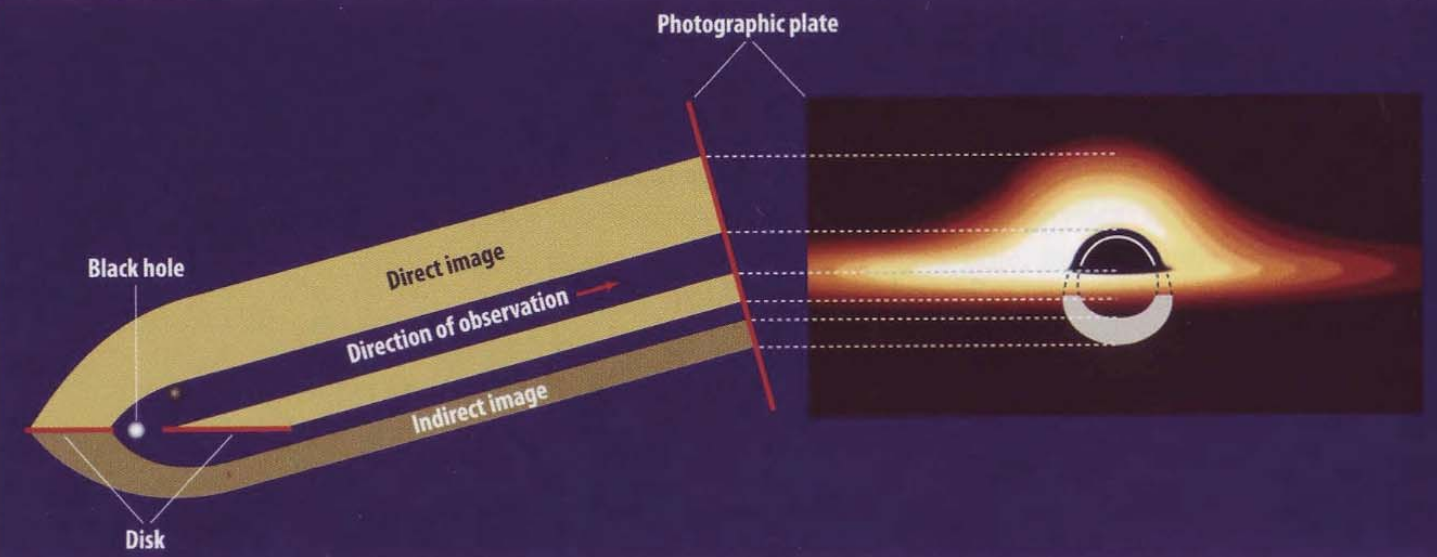
\includegraphics[width=\columnwidth]{Images/lensed_cartoon}
\caption{(Image credit : Shep Doeleman) Cartoon image (left) combined with the ray-tracing of a thin accretion disc surrounding a BH, first calculated by \citet{Luminet_1979}. The cartoon image shows that both the bottom and top of the back of the accretion disc is lensed by the black hole and becomes visible The dark area in the centre, known as the black hole shadow is the lensed image of the photon ring orbiting the BH. A measurement of it's precise shape is a test of general relativity in the strong field regime. Note that the left-right asymmetry in the image is due to doppler boosting, and that all sides of the accretion disk and photon ring are visible due to lensing. \label{fig:grmhd}%
}
\end{center}

\end{figure}



\subsection{Space-time in strong gravity}

%Probing strong gravity and black hole spacetime St 1
Gravity as described by General Relativity (GR) is consistent with all observational experiments thus far, however GR has conceptual weaknesses, especially as it is not compatible with the quantum description of reality. Various alternatives to GR have been theorised which do not assume a purely classical description of matter. To compare GR with the alternatives, we have to compare its predictions in the strong, non-linear field regime where the largest deviations from GR would occur if it were an approximate theory.


The spacetime within several $R_g$ around a SMBH provides this opportunity. The precise shape of the the photon ring around a SMBH is dependent on the spacetime which in turn is calculated within a theory of gravity \citep{Takahashi_2004}. The No-Hair theorem, which is based on GR, states that the spacetime should only be determined by the first two moments of the black hole, i.e. it's mass and spin. If the No-Hair theorem is invalid, the ring will deviate from a Schwarschild or Kerr profile. In the case of a non-zero quadrupole moment the ring will become either oblate or prolate \citep{Johannsen_2010}. This asymmetry is potentially measurable by EHT observations \citep{Broderick_2014}.

Is there an event horizon or a surface? - surface would radiate


\section{Cranking up the angular resolution}

%Increasing resolution -> motivation and difficulties
Throughout the history of astronomy, there have been celestial sources which appear point-like (unresolved) with the available instrumentation. To investigate the nature of these sources, ever more sophisticated instruments with higher resolution are developed. 

In principle, a diffraction-limited aperture can obtain an angular resolution of
\begin{equation}\label{eq:ang_res}
 \theta_{\rm res}\ \approx \ 1.22\ \lambda / D,
\end{equation}
where $D$ is the diameter of the aperture and $\lambda$ is the observing wavelength. However, dish apertures larger than a hundred metres are infeasible to construct while systematic errors, including scattering-induced blurring due to inhomogeneous density (radio) or temperature (optical) distributions in the Earth's atmosphere can lead to instrument being unable to reach the diffraction limit. To overcome these difficulties and improve $\theta_{\rm res}$, a variety of new technologies have been developed (see Fig~\ref{fig:spec_ang}), including space-based observatories which escape the limitations set by the Earth's atmosphere, interferometric arrays which eliminate the need to build extremely large apertures, as well as technology-enabled mitigation strategies like adaptive optics and water vapour radiometry which account for atmospheric turbulence in real time. 


%Very Long Baseline Interferometry -> the highest resolution
The observing technique which typically achieves the highest angular resolution is Very Long Baseline Interferometry (VLBI). Interferometry refers to the technique of measuring the electric field correlations (named `visibilities') between pairs of separated antennae. The visibilities are related to Fourier components on a section of approximately flat sky. Through an `adequate' sampling of the Fourier domain an approximate image of sky can be reconstructed using the inverse Fourier transform. With this method, the distance between the antennae ($\bm{b}$, referred to as the `baseline') effectively replaces $D$ in equation~\ref{eq:ang_res}, yielding a higher angular resolution than a single aperture. This technique is primarily used at radio frequencies while the electric field phase remains relatively stable. VLBI is essentially radio interferometry with antennae separated by large distances, typically $\gtrsim 100$~km, including the possibility for antennae in Earth's orbit. A key distinction from connected-element interferometery is that independent clocks are needed at each station to facilitate the post-observation correlation. VLBI has seen several noteworthy achievements since its inception in the late 1960's, including resolution of the extra-galactic, compact, highly-variable objects, now known as quasars into super-luminal core-jet systems \citep[e.g.][]{Whitney_1971}, and the mapping of maser motion around the Super-Massive Black Holes (SMBH) in the cores of nearby galaxies \citep[e.g.][]{Miyoshi_1995}.


%fig : angular resolution across spectrum
\begin{figure}
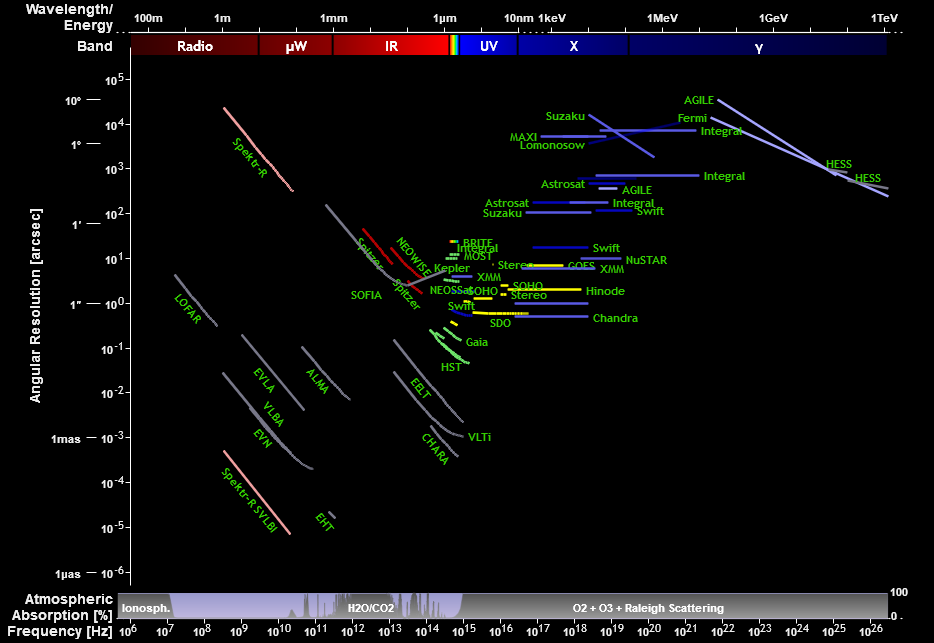
\includegraphics[width=\columnwidth]{Images/spec_ang}
\caption{(Image credit: Olaf Frohn\protect\footnote{http://armchairastronautics.blogspot.co.za/p/space-observatories.html}) An illustration of angular resolution vs. observing frequency across the entire observational spectrum, shown for a selection of observatories. The VLBI arrays : Spektr-R SVLBI (or RadioAstron) and the EHT clearly achieve the highest angular resolution of all due to their long baselines. At the bottom of the plot, there is a panel showing atmospheric/ionospheric absorption as a function of wavelength, and consequently all observatories in the zero transmission zones are space-based. \label{fig:spec_ang}
}
\end{figure}

As will be described in the next section, the ultra-high angular resolution provided by VLBI enables investigation into several key questions concerning black holes.



\section{The Event Horizon Telescope}
\subsection{Overview}

% EHT -> intro to the Array st 1
In the last few decades there has been a push to enhance VLBI capabilities at sub-millimetre wavelengths. One of the leading efforts in this regard is the Event Horizon Telescope consortium \citep[(EHT),][]{Doeleman_2010}, an international project whose primary objective is to spatially resolve the lensed photon rings nearby SMBHs with an angular resolution on the order of their event horizons. In contrast to competing high frequency VLBI observatories e.g. the Very Long Baseline Array (VLBA) which had coverage to 87~GHz (3~mm), the EHT is operating at 230~GHz (1.3~mm) and will potentially extend till 345~GHz (0.8~mm) in the future. See Fig.~\ref{fig:eht_globe} for an annotated map of the locations of the EHT array. As the EHT will have baseline lengths comparable to the diameter of the earth, $|b| \sim 10^4$~km and is operating at 1.3~mm, this yields $\theta_{\rm res} \sim 30\ \mu$-arcsec.

%st 1
\begin{figure}
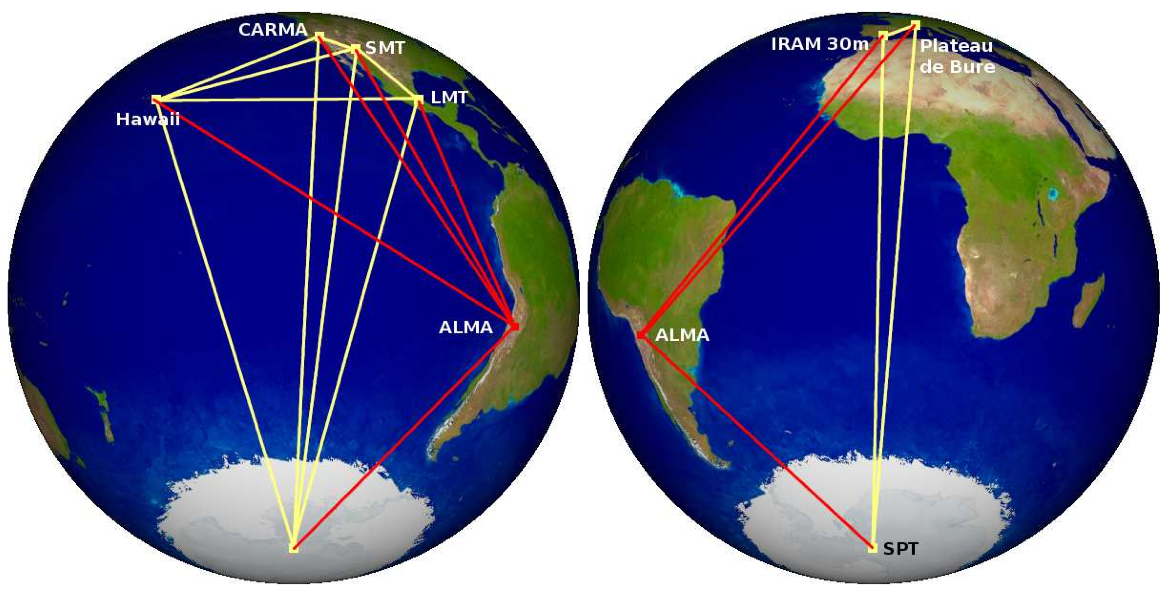
\includegraphics[width=0.8\columnwidth]{Images/eht_globe}
\caption{(Image credit: Remo Tilanus) The view of the Event Horizon Telescope (EHT) from Sgr~A*. This interferometric array uses Earth-diameter baselines, operating at $230-345$~GHz to attain an angular resolution of the order of ${\theta_{\rm res} \sim 10\ \mu}$-arcsec. Baselines to ALMA are shown in red, to highlight its order of magnitude higher sensitivity. Note that the CARMA station has recently been decommissioned, a telescope in Greenland is currently being constructed and there is ongoing investigation into a possible site on the African continent.\label{fig:eht_globe}%
}
\end{figure}



\subsubsection{Instrumentation and observational challenges}

%intro - newness of field and instrument st 1
The development of mm-VLBI instrumentation has been spurred by the formation of EHT as a project and the deepening of theory and simulation work over the past two decades. This is evidenced by the comparable observational results but starkly different interpretations of \citet{Krichbaum_1998} and \citet{Doeleman_2008}. A decade apart, both teams observed Sgr~A* with a mm-VLBI arrays consisting of three stations at similar frequency (215~GHz in 1998 and 230~GHz in 2008). Although the former was limited by calibration problems, the primary difference in analysis and interpretation was that the later result was linked explicitly to the innermost accretion physics in the event horizon region \citep[e.g.][]{Broderick_2011} i.e. the newly developed theoretical context contributed to the significance of the \citet{Doeleman_2008} result. However, to robustly interrogate this diverse body of theoretical work, an ultra-high precision instrument is needed. For example, to discern whether the No-Hair theorem is violated requires the fractional asymmetry of the shadow shape with respect to its angular size to be measured to a few percent \citep{Goddi_2016}. To achieve this level of precision, the development of the global mm-VLBI array will surely be faced with its fair share of obstacles.

%St : 1

%moving to higher freq st1
The move to higher frequencies is accompanied by requirements on the instrument including: increased data rates and stability of timing standards; as well as increased accuracy of dish surfaces and antenna pointing accuracy. Difficulties emerge also from the effects of the Earth's lower atmosphere where optical depth becomes significant and turbulence causes rapid fluctuations in the signal transmission time which causes decoherence in the visibilities. Even though the stations are in high altitude, desert locations, the atmospheric coherence times are still short, typically $\lesssim$10~s \citep{Doeleman_2009}. The extensive requirements on instruments and location push up the cost of mm-VLBI stations resulting in sparsely populated interferometric arrays which make for inadequate sampling of the Fourier domain. 




%More complicated effects
Aside from the considerations listed above, there are other important issues relevant to the target sources, the ISM and the calibration procedure. Firstly the line-of-sight to the Galactic Centre passes through an inhomogeneous turbulent electron plasma in the Interstellar Medium (ISM). This medium both blurs and introduces random, time-variable substructure into the source brightness distribution (see section~\ref{sec:ism_scat}). The scattering substructure adds substantial complications for data interpretation as its contribution is difficult to entangle from that of the intrinsic source substructure. The second issue is that the source itself is variable over minutes to hours (see section~\ref{sec:variability}). The fact that the source is variable over the course of a single observation epoch breaks a fundamental assumption in interferometry as the visibilities cannot be related to a single sky image. Additional complications arise due to the assumptions in self-calibration that the source is static, while in fact both the source and the ISM are time-variable. Traditional calibration is also difficult as the high frequency sky has a lower calibrator source density and calibrators are mostly resolved and possible variable too. 


% Effect of corruptions on Science extraction : parameter estimation and imaging, #HighAccuracy
These effects, among others, may place significant limitations on the sensitivity, image fidelity, and dynamic range that can be achieved with mm-VLBI.  Furthermore, unaccounted for systematic and/or non-Gaussian uncertainties could preclude robust, accurate Bayesian parameter estimation and model selection analyses of accretion flow \citep[e.g.][]{Broderick_2016} and gravitational physics \citep[e.g.][]{Broderick_2014, Psaltis_2016}, two of the EHT's many objectives. 


\section{A realistic mm-VLBI simulator}
%Pr : 1 : St : 1

%Why simulate: intro 
Given the significant observational challenges that the EHT faces, we have undertaken this project to build a mm-VLBI observation and signal corruption simulator. There are many benefits for using such a toolkit and indeed synthetic data simulation is common practice for major scientific experiments. A prominent example is the extensive gravitational wave template matching scheme for The Laser Interferometer Gravitational-Wave Observatory (LIGO) which operates in the presence of tidal loading, passing trains etc. In essence such a simulator would fill in the final component of the theoretical signal propagation chain, effectively taking astrophysical simulations of the source (e.g. accretion onto a SMBH) as an input and returning realistic synthetic interferometric data. This allows a more effective interplay between theory and observation, quantifying systematic effects and the measurement limits. The remainder of this section will briefly discuss several research questions relevant to an EHT synthetic data simulator and how we approach the software design in order to address these questions. 

%Specific use cases of simulations

%Testing calim through standard challenges 
A key use case for simulated data is the testing of calibration, parameter estimation and imaging algorithms and strategies. As the inputs to the simulator are known exactly, we are better able to explore sources of error which are difficult to disentangle from intrinsic source features when using only real data. A straightforward way to perform such a test is through the creation of a set of `standard challenge' dataset. Such datasets would be available to the entire community to input into their calibration and/or imaging routines. Following this, a detailed comparison between the different strategies in varying regimes (source, ISM, troposphere and instrumental) can be made. Importantly, a systematic investigation of a particular algorithm across many different datasets could provide insight into subtle or previously unknowns sources of error inherent in that routine.


%Optimising observations 
Simulated data can also assist in the optimisation of the experimental configuration. Financial constraints require the prioritisation of hardware upgrades e.g. increasing bandwidth, surface accuracy improvement, deployment of water vapour radiometers or additional receiver bands. Simulated data together with calibration and imaging pipelines can help to quantify the benefit of each improvement based on expected scientific return in units of precision of the scientific parameter of interest (e.g. shadow assymetry) rather than more generic terms (e.g. angular reso. This approach can even be extended to assess new candidate stations, especially as new geographic locations e.g. in Southern Africa are receiving increasing attention due to the potential long baselines to ALMA, SPT and European stations.


%other simulation efforts 
Recently, there has been an increase in the attention given to simulating EHT observations of Sgr~A*  and M87 \citep{Fish_2014,Lu_2014,Bouman_2015,Lu_2016,Chael_2016}. However, these are primarily focused on image reconstruction and assume either negligible or Gaussian distributed gain errors; perfect antenna pointing accuracy; and in most cases only Gaussian convolution to simulate ISM scattering. Clearly, as the EHT array is enhanced (and possibly expanded), so too must the interferometric simulations evolve to provide ever-more physical predictions on the confidence levels with which parameters can be extracted and hence exclude theoretical models of gravity and/or accretion flows.


%the Meqtrees+MS approach
Over the past decade, significant effort has been placed on advanced radio interferometric calibration and imaging algorithms for centimetre and metre-wave facilities in response to the large number of new arrays in construction or design phase (e.g. MeerKAT, ASKAP, SKA, LOFAR, HERA). A leading software package in this pursuit is \textsc{MeqTrees}\footnote{https://ska-sa.github.io/meqtrees/} \citep*{Noordam_2010}, which was developed to simulate, understand and address the calibration issues to be faced with the greatly enhanced sensitivity, instantaneous bandwidth, and field-of-view of such facilities. For example, \textsc{MeqTrees} is rooted in the Measurement Equation mathematical formalism \citep{Hamaker_1996}, which parameterizes the signal path into distinct $2 \times 2$ complex  matrices called Jones matrices. This formalism and applications thereof are laid out in \citep{Smirnov_2011a,Smirnov_2011b,Smirnov_2011c} and are arbitrarily generalized to model any (linear) effect, including undesired signal corruptions that often may have subtle yet systematic effects. \textsc{MeqTrees} has been applied to correct for direction dependent calibration errors to JVLA and WSRT observations, achieving record-breaking high dynamic range images \citep{Smirnov_2011c}. The effectiveness provided by the Measurement Equation formalism in radio interferometric calibration provides a strong motivation to explore its application to challenging goal of imaging a supermassive black hole silhouette with mm-VLBI. To construct this simulator we leverage off metre and cm-wavelength simulation and calibration successes and build a \textsc{MeqTrees}-based mm-VLBI-specific software package which we name, \textsc{MeqSilhouette}.  Use of \textsc{MeqTrees} and \textsc{measurement set} data format lends itself to investigating a range of different techniques that are used in other areas of interferometry (e.g. coh-Jones paper). While \textsc{MeqTrees} has not yet been used in the context of mm-wavelength observations, the framework is agnostic to higher frequency implementation as long as the Measurement Equation is appropriately constructed. 


\section{Outline}

This thesis is broadly divided into the following chapters and sections,
\begin{itemize}
 \item {\bf Chapter 2 : Theory} 
 \begin{description}
  \item [Section 2.1] introduces radio interferometry via the Measurement Equation formalism, followed by a brief discussions on a selection of topics relevant to mm-VLBI.
  \item [Section 2.2] is a review and investigation into the key signal corruptions to be implemented in our proposed mm-VLBI simulator.
 \end{description}

 \item {\bf Chapter 3 : Software Implementation}\\
 A description of the design and construction of the simulation software with emphasis on the software architechure and workflow.
 
 \item {\bf Chapter 4 : Results and Analysis}
 \begin{description}
  \item  [Section 4.1] showcases the basics of the simulator output through a series of canonical results.
  \item [Section 4.2] is a more sophisticated scenario involving calibration in ..
 \end{description}
  
  \item {\bf Chapter 5 : Conclusions and future work}\\
  We summarise the work and context of this thesis as well as make suggestions for future applications and improvements.
 
\end{itemize}

















%\chapter{Theory}\label{chap:theory}
%plan st 1
In this chapter we review and develop the theory required to model signal transmission from cosmic source to uncalibrated (raw) interferometric data. The first half of this chapter provides the necessary introduction to fundamental radio interferometric concepts while the second half is focused specificially on describing several key signal corruptions, relevant to mm-VLBI observations. 

\section{Radio Interferometry}\label{sec:radio_int}
%St 2

%plan st 1
This section is structured as follows: first radio interferometry is introduced using the Radio Interferometric Measurement Equation (RIME) formalism, which serves as a guiding framework for the construction of the {\sc MeqSilhouette} simulator. We then review the technique of self-calibration, typical mm-VLBI data products and the consequences of breaking the static source assumption.

\subsection{Measurement Equation}\label{sec:RIME}
%PR 2 St 1

%RIME intro and purpose
The RIME provides the notation and formalism to model the signal transmission path as a sequence of linear operations. It takes into account polarisation, correlation and the correct time-ordering of signal transmission path in an intuitive and efficient way. The formalism also enables a more informative phrasing of the relation between calibration and signal corruptions.


%Linear transformations of E-field
Here we offer a short derivation and explanation of the RIME following \citet{Smirnov_2011a}. Consider a quasi-monochromatic, complex-valued electric field vector $\bm{E}$, which can be decomposed into an arbitrary two dimensional orthogonal basis in the plane perpendicular to the direction of propagation,

\begin{equation*}
\bm{E} = \left(
\begin{array}{c}
E_a \\
E_b \\
\end{array} \right),
\end{equation*}
\noindent where this choice represents the basis in which the polarisation is measured. All linear transformations of the above electric field can be written by a multiplication with a 2 x 2 complex valued matrix, termed a \emph{Jones} matrix \citep{Jones_1941}[ads was down!],
\begin{equation}
\bm{E'} = \bm{J E}.
\end{equation}
For example, the conversion of the electric field to a voltage $\bm{v}$ at an antenna can be specified by such a transformation i.e. $\bm{v} \equiv \bm{E'}$ under multiplication with the appropriate $\bm{J}$. Multiple effects then can be represented by multiplication of various Jones matricies, forming a Jones chain,
\begin{equation}
\bm{E'} = \bm{J}_n \ldots \bm{J}_1\ \bm{E}.
\end{equation}

%More on Jones matricies: commutivity and order, DDE vs DIE. phenomenological vs. physical
The order of the Jones matricies should obey the casual order of the signal transmission path (i.e. $\bm{J}_1$ would closest to source, $\bm{J}_n$ closest to antenna). However the rules of commutivity of matricies allows us some flexibility. Matricies which are scalar commute with everything, while diagonal matricies commute with each other as do matricies which effect a rotation of $\bm{E}$. This allows the Jones chain to be re-ordered into more convienent formulations as required. In other words, the signal path can parameterised in different ways. For example during calibration, it is useful to contruct a \emph{phenomenological} Jones matrix which represents the combined action of several \emph{physical} commuting processes/matricies (e.g. ionospheric delay and electronic drift). The advantage would be that only the cumulative effect is considered, which keeps the number of parameters to solve for to a minimum. This would be useful when the individual effects cannot be easily distingushed and/or have the same Jones matrix form. On the other hand, for realistic data simulation, we prefer to model the signal transmission path by formulating a Jones matrix based on the exact physical process.


%visibility definition
An interferometer measures the correlation of the voltages from an antenna pair, referred to as a  \emph{baseline}. The correlator output is termed the \emph{visibility}, 
\begin{equation}
\bm{V}_{pq} = \langle {\bm v}_p  {\bm v}_q^H \rangle,
\end{equation}
where $p$, $q$ are refer to the two antennae. The representation of  $\bm{V}_{pq}$ as a 2~x~2 matrix is equivalent to the Stokes polarisation formulation, for example in an XY basis,


%Connection to stokes parameters and polarisation
\begin{eqnarray}
\bm{V}_{pq} &= & \bm{J}_p \langle {\bm E}_p  {\bm E}_q^H \rangle \bm{J}_q^H \\
&=&  \bm{J}_p\left(
\begin{array}{cc}
\langle E_{xp} E_{xq}* \rangle & \langle E_{xp} E_{yq}* \rangle \\
\langle E_{yp} E_{xq}* \rangle & \langle E_{yp} E_{yq}* \rangle \\
\end{array} 
\right) \bm{J}_q^H \\ 
&=&
 \bm{J}_p \left(
\begin{array}{cc}
I+Q & U +iV\\
U-iV & I-Q \\
\end{array}
\right)\bm{J}_q^H,
\end{eqnarray}
where $I$ is the coherence of the total flux, $V$ is the coherence of the circularly polarised flux, $Q$ and $U$ relate to coherence of the linear polarisation. Note that the Jones matricies are assumed to be constant over the time and frequency averaging interval. As this formalism is coordinate system independent, we can easily transform any 2~x~2 from a linear to circular basis and vice-versa. 

% Example RIME and re-derivation of van-citterlike
We now review the RIME for a single, uncorrupted, unpolarised point source, which will illustrate the Fourier transform relation between the measured visibility and a section of approximately flat sky.
%phase diff
Considering that there are no signal corruptions, the only Jones matrix to consider is the effect of the phase difference of the electric fields measured at the two antennae. This is due to the difference in propagation path length.


%coordinate systems
Consider the vector $\bm{\sigma}$ which points from the centre of the Earth towards the source. We define the position difference between the two antenna or baseline vector $\bm{u} = (u,v,w)$ with the w-axis in the direction of $\hat{\bm{\sigma}}$. Next we denote the angular position on the sky by $(l, m)$ which are the directional cosines on the sky measured in the direction of $(u, v)$ respectively. Note that we consider only a small approximately flat section of the celestial sphere centred on $\bm{\sigma}$, also called the \emph{phase centre}. The phase difference between rays arriving at the two antennae is therefore,
\begin{equation}
 \delta \phi = 2\pi (\bm{u}/\lambda \cdot \bm{\sigma})
\end{equation}

As we are only interested in a small, approximately planar component of the sky (i.e. $l^2 +m^2 \ll 1$),
\begin{equation}
 \delta \phi \approx 2\pi \lambda^{-1} (u_pl +v_pm).
\end{equation}
Denoting the brightness matrix $\bm{B} = \langle {\bm E}_p  {\bm E}_q^H \rangle$ and setting the delay of antenna $q$ as the reference, the RIME for our simplified model becomes
\begin{eqnarray}\label{eq:van-citterlike}
\bm{V}_{pq} &=& K_p \bm{B} K_q^H \\
&=&  \exp (2\pi i \lambda^{-1} (ul +vm)) \bm{B} (1)
\end{eqnarray}
where $K$ was the Jones matrix used to apply the phase difference to each antenna. This is a Fourier Transform relation between visibility domain $(u,v)$ and image domain $(l,m)$. This derivation can be easily broadened to include extended sources (e.g. see \citep{Smirnov_2011a}). The quantity  $K_p \bm{B} K_q^H$ is often denoted as $\bm{X}_{pq}$ and is termed the coherency matrix.


%example signal corruption, Complex time-variable antenna gain
An example of a Jones matrix representing a signal corruption is the complex time-variable antenna gain. Considering two independent linear dipoles,  for antenna p
\begin{equation}\label{eq:G_jones}
\bm{G}_p(t) =
\left(
\begin{array}{cc}
g_x (t)&0\\
0 & g_y (t) \\
\end{array}
\right)
\end{equation}
Hence the RIME in this case becomes,
\begin{equation}\label{eq:G_rime}
\bm{V}_{pq} = \bm G_p \bm{X}_{pq} \bm G_q^H
\end{equation}

\subsection{Self-calibration and fringe fitting}\label{sec:self_cal}
%Pr 2 St 1
Self-calibration, as the name suggests, uses the target itself as a calibrator to estimate station gains.
In mm-VLBI calibration, self-calibration is applied under two different formulations. The first is a procedure termed \emph{fringe fitting}.
%Self-calibration proper
The second formulation of self-calibration (which I will just refered to as self-calibration) is to iteratively solve for station gains but not their derivatives whilst constructing the sky model. We begin with the initial sky model (typically a point source) as well as the station gains output by the fringe fit. Then we solve equation~\ref{eq:G_rime} using a least squares procedure but without taking into account station gain phase derivatives so that there are fewer free parameters. The resulting dataset is then imaged, deconvolved (i.e. the effect of the synthesised beam is removed) and a source finder is applied on the image to construct a more accurate sky model. This sequence is then repeated with the updated sky model being used when solving for station gains. The loop will terminate when a specified flux threshold is reached.

%fringe fitting
 From the point of view of the RIME, fringe-fitting solves for station gains in equation~\ref{eq:G_rime} over a time interval typically on the order of minutes. Taking a linear expansion in frequency and time of the phase of the station gain yields,

\begin{IEEEeqnarray}{rCl}
\bm{V}_{pq}(t_0,dt,\nu_0,d\nu)& = & |G_p||G_q| \bm{X}_{pq} \exp(i[\phi_p(t_0,\nu_0)  + \partial_t \phi_p(t,\nu_0)dt \nonumber\\
&& \negmedspace {} + \partial_\nu \phi_p(t_0,\nu)d\nu  -\phi_q(t_0,\nu_0) -  \nonumber\\
&& \negmedspace {} \partial_q \phi_p(t,\nu_0)dt - \partial_\nu \phi_q(t_0,\nu)d\nu]).
\end{IEEEeqnarray}\label{eq:fringe_fit}

A blind search is then performed for all the station based parameters in the above equation i.e. everything except $\bm X_{pq}$. The station gain amplitude will sometimes be calibrated separately, reducing the number of parameters to solve. The sky model used is typically just a point source at the centre of the field. 





The interaction of both fringe fitting and self-calibration with a variable source, tropospheric, ISM and instrumental signal corruptions is of central interest to this investigation.


\subsection{mm-VLBI observables and data products}
%PR 2 St 1

%Visibility amplitudes, closure quantities, polarisation ratios, and images.
If the visibility phase is highly variable as in the case of a turbulent atmosphere,  conventional calibration and imaging techniques have severely limited (if any) success. However information can still be extracted from the raw visibilities in the form of closure quantities \citep{Monnier_2007} or polarisation ratios \citep{Fish_2009}. Visibility amplitudes are also used although they suffer from systematic errors, a subset of which are dealt with in this work. There also exist imaging algorithms \citep[e.g.][]{Lu_2014,Bouman_2015,Chael_2016} which use closure phase as a regulariser to ensure that miscalibration of station gains do not effect the resulting image, although these unconventional imaging algorithms come with their own uncertainties on fidelity. Closure phase, defined as the sum of 3 visibility phases of a triangle of stations $\left\{i,j,k\right\}$, is a probe of point-asymmetry in source structure,
\begin{equation}
\Phi_{ijk} = \phi_{ij}+\phi_{jk}+\phi_{ki}.
\end{equation}

\noindent Because most signal corruptions are station based, the gain phase terms $\phi_{ij}=\phi^{\rm true}+ \phi^G_i -\phi^G_j$ for each antenna, assuming constant over the integration time and bandwidth will cancel, yielding a more robust observable.  

In the literature, the uncertainty on the closure phase is calculated in various ways. One method is model dependent \citep{Rogers_1995} and is given as a function of the SNR $s$ of each baseline 

\begin{equation}\label{eq:ucp}
u(\Phi_{ijk}) = \frac{\sqrt{4 + (s_{ij}s_{jk})^2 + (s_{jk}s_{ki})^2 + (s_{ij}s_{ki})^2 +
                        2(s_{ij}^2+s_{jk}^2+s_{ki}^2)}}{s_{ij}s_{jk}s_{ki}},
\end{equation}

\noindent where $s_{ij}$ is defined as
\begin{equation}
s_{ij}=|V_{ij}| \sqrt{\frac{ \tau \Delta \nu}{SEFD_i SEFD_j}},
\end{equation}
where $\tau$ is the vector averaging timescale, $\Delta \nu$ is the bandwidth, $|V_{ij}|$ is the visibility amplitude and $SEFD$ is the system equivalent flux density.

Alternatively, assuming Gaussian errors the uncertainty on the closure phase over a scan $u(\Phi_{ijk})=\sigma(\Phi_{ijk})/\sqrt(n)$  \citep{Brinkerink_2016}.

\subsection{Variability and the static source assumption}\label{sec:variability}
%PR 1 St 1

%the assumption and how it breaks the image-vis fourier transform relation
Implicit in our description of interferometry above (e.g. equation~\ref{eq:van-citterlike}), we assumed that the source remains approximately unchanged or static during the course of the observation. However, if this assumption does not hold (i.e. if the source is time-variable), the visibilities measured over the course of an observation can no longer be related to a single image.
%explicitly defining variability as any intrinsic source variability
Note that I am using the term `variability' in a general sense which refers to changes in any source observables. 'Variability' is most often used to denote changes in source flux but we extend the definition to include changes in source structure, position and polarisation.
%expectation & calim
We expect that an image of a variable source would appear smeared out as it is averaged over many realisations and that ghosts should arise during the calibration/deconvolution procedure {\bf [citations? trienko's papers?]} . One of the objectives of this thesis will be to characterise the errors which emerge when a variable source is self-calibrated in the presence of troposheric-induced errors. Practically it is difficult to separate source and instrumental variability without accurate models for both. 


%Observed variability from SgrA
Although the static source assumption holds for most interferometric observations, the accretion flow and/or magnetic field structures around a SMBH can be variable on far shorter timescales. The primary mm-VLBI target, Sgr~A*,  exhibits variability on timescales of minutes to hours in the radio (including EHT observations), near-infrared (NIR), and X-ray bands \citep[e.g.][]{Baganoff_2001, Genzel_2003, Yusef-Zadeh_2006, Maronne_2006, Fish_2011, Johnson_2015b}. This wealth of observational data has yielded several answers but the origin of the variability is still highly debated. To explain the observed delays between flares in different frequency bands, an expanding adiabatic plasma model (Marrone, 2008) has been presented however a recent flare observed with the EHT did not exhibit the increase in size expected from an expanding plasma outflow model \cite{Fish_2011}.  Signatures of periodic variability at NIR and x-ray \citep{Genzel_2003; Belanger_2006} have been used to argue for the presence of orbiting hotspots \cite{Doeleman_2009}. As the Innermost Stable Circular Orbit (ISCO) depends on spin of the BH, the spin can be constrained through the detection periodic orbital features. On the other hand, a more recent observation of a longer light curve in the NIR is more representative of a power-law scale variability \cite{Meyer_2008}. The cumulative evidence of these observations point to the possibility of multiple flaring mechanisms. An important mm-VLBI observational result is that variability in the polarisation domain is far more rapid than the total intensity (Johnson 2015b), indicating that the magnetic fields structure is highly dynamic.


%Light crossing analysis
In principle, the variability timescale could be comparable to the period of the Innermost Stable Circular Orbit (ISCO), which for Sgr~A$^\star$, ranges from 4 minutes in the case of a maximally rotating BH with a prograde disc to about half an hour for a non-rotating BH. The ISCO period for M87 is substantially longer, on the order of days [refs]. Considering light crossing times $\Delta t_{\rm cross}$, we can estimate the angular size $\theta$ of the emission region to be of order $\theta \sim \Delta t_{\rm cross} c /D_{\rm src}$, where c is the speed of light and $D_{\rm src}$ is the observer-source distance. Hence for Sgr~A* at $D_{\rm src} = 8.3$~kpc (Gillessen, 2009), a flare of duration $ \Delta t_{\rm cross} =10$~min corresponds to scales of  $15 R_{\rm Sch}$. Such analyses gave early evidence for an emission area on event horizon scales.


%There are some ways to track/mitigate variability but this is beyond scope
In the case of a highly localised flare, several approaches \citep{Doeleman_2009, Fish_2009b, Johnson_2014} show that EHT can track such a structure with $\sim 5\ \mu$-arcsec precision using closure quantities and polarimetric ratios. This could help map the spacetime around the BH. Alternatively \citet{Lu_2016} show that a gaussian weighting scheme can be applied to mitigate the effects of variability and measure the quiescent structure although this approach would downweight the longest baselines. However all of these approaches assume only gaussian thermal noise, guassian-blurring in the ISM and no tropospheric-induced calibration errors.

\section{Signal Corruptions}
%plan
We begin with an introduction to scattering theory, which is applicable to the radiative processes occuring in both the troposphere and ISM. Following this we explore signal corruptions due to the transmission through the ISM and Earth's atmosphere as well as instrumental imperfections in detail. 

\subsection{Scattering basics}\label{sec:basic_scat}
%PR 1 St 1

%motivation
Millimetre wavelength radiation originating at the Galactic Centre is repeatedly scattered along the signal path to the Earth-based observer. The first occurrence is due to electron plasma in the ISM \citep[e.g.][]{Bower_2006,Gwinn_2014}, while the second is due to poorly-mixed water vapour in the Earth's troposphere \citep*[e.g.][]{Carilli_1999, Lay_1997}. It is essential that the effects of the scattering phenomena are understood for accurate calibration and robust inference of the intrinsic source properties.  To this end, simulation modules approximating scattering in both media are implemented in \textsc{MeqSilhouette}. As an introduction to the separate descriptions of each, we review a simple scattering model.

%description of the model
An electro-magnetic wave is scattered when it passes through a medium with refractive index inhomogeneities. Following \citet{Narayan_1992}, this effect can be modeled as a thin screen, located between source and observer planes and orientated perpendicular to the line-of-sight. The screen, indexed by coordinate vector $\mathbf{x}$, adds a stochastic phase $\phi(\mathbf{x})$ to the incoming wave at each point on the screen, yielding a corrugated, outgoing wavefront. We define the Fresnel scale as  $r_{\rm F} = \sqrt{\lambda D_{\rm os}/2\pi}$, where $D_{\rm os}$ is the observer-scatterer distance, or the distance where the geometrical path difference $\frac{2\pi}{\lambda} (D_{\rm os} - \sqrt{D_{\rm os}^2 + r_{\rm F}^2}) =\frac{1}{2}$~rad.

%example calculation
To determine the resultant electric field at a point in the plane of the observer, indexed by coordinate vector $\bm{X}$, one has to take into account all possible ray paths from the screen to $\bm{X}$. To illustrate the model, a calculation of the scalar electric field generated by a point source, $\psi(\bm{X})$ yields the Fresnel-Kirchoff integral \citep*{BORN_1980}
\begin{equation}\label{Fresnel- Kirchoff}
\psi(\bm{X}) = C \int_{\rm screen} \exp\left[i\phi(\bm{x}) + i \frac{(\bm{x}-\bm{X})^2}{2 r_{\rm F}}\right]\bm{dx},
\end{equation}
where C is a numerical constant.

%define structure function
The statistical properties of $\phi(\mathbf{x})$ can be described by a power spectrum or equivalently the phase structure function,
\begin{equation}\label{eq:D_phi}
D_\phi (\mathbf{x},\mathbf{x'}) = \langle \left[ \phi(\mathbf{x} +\mathbf{x'}) - \phi(\mathbf{x})\right]^2 \rangle,
\end{equation}
where $\mathbf{x}$ and $\mathbf{x'} $ represent two points on the screen and $\langle .. \rangle$ denotes the ensemble average. 

There is evidence that $D_\phi$ can be reasonably approximated by a power law dependence on the absolute distance $r$ between points on the screen  \citep{Armstrong_1995,carilli_1997}
\begin{equation}
D_\phi (r) =  (r/r_0)^\beta,\qquad r^2 = (\mathbf{x} - \mathbf{x'})^2
\label{kolmogorov}
\end{equation}
where $r_{\rm 0}$ is the phase coherence length scale defined such that $D_\phi(r_{\rm 0}) = 1$~rad. 
%kolmogorov turbulence
Kolmogorov turbulence, which describes how kinetic energy injected at an outer length scale $r_{\rm out}$ cascades to increasingly smaller scales until finally dissipated at an inner length scale $r_{\rm in}$, predicts $\beta = 5/3$ in the domain ${r_{\rm in}<<r<<r_{\rm out}}$. This scaling has been demonstrated to be a reasonable approximation for the ISM over scales $r \sim 10^2$~km to $>1$~AU \citep*{Johnson_2015a}, and also for the troposphere with $r< \Delta h$, where $\Delta h$ is the thickness of the turbulent layer \cite{Coulman_1985}. The specifics of the tropospheric model will be explored further in later sections.

%Weak and strong
The two length scales, $r_{\rm F}$ and $r_{\rm 0}$, define the nature of the scattering which is split into the strong and weak regimes, Fig.~\ref{fig:scatter}. In weak scattering, $ r_{\rm 0} \gg r_{\rm F}$ and hence by equation\ ~\ref{kolmogorov}, $D_{\phi}(r_{\rm F}) \ll 1$. This implies that most of the radiative power measured on a point $\bm{X}$ will originate from a screen area $A_{\rm weak} \approx \pi r_{\rm F}^2$. Whereas in the regime of \emph{strong scattering}, $ r_{\rm 0} \ll r_{\rm F}$ yielding  $D_{\phi}(r_{\rm F}) \gg 1$. This  results in coherent signal propagation onto the point $\bm{X}$ from multiple disconnected zones each of area $A_{strong} \approx \pi r_{\rm 0}^2$ \citep{Narayan_1992}. Scattering in the troposphere and ISM in the direction of the Galactic Centre fall into the regimes of weak and strong scattering respectively.

%Weak and strong fig
\begin{figure*}
\begin{center}
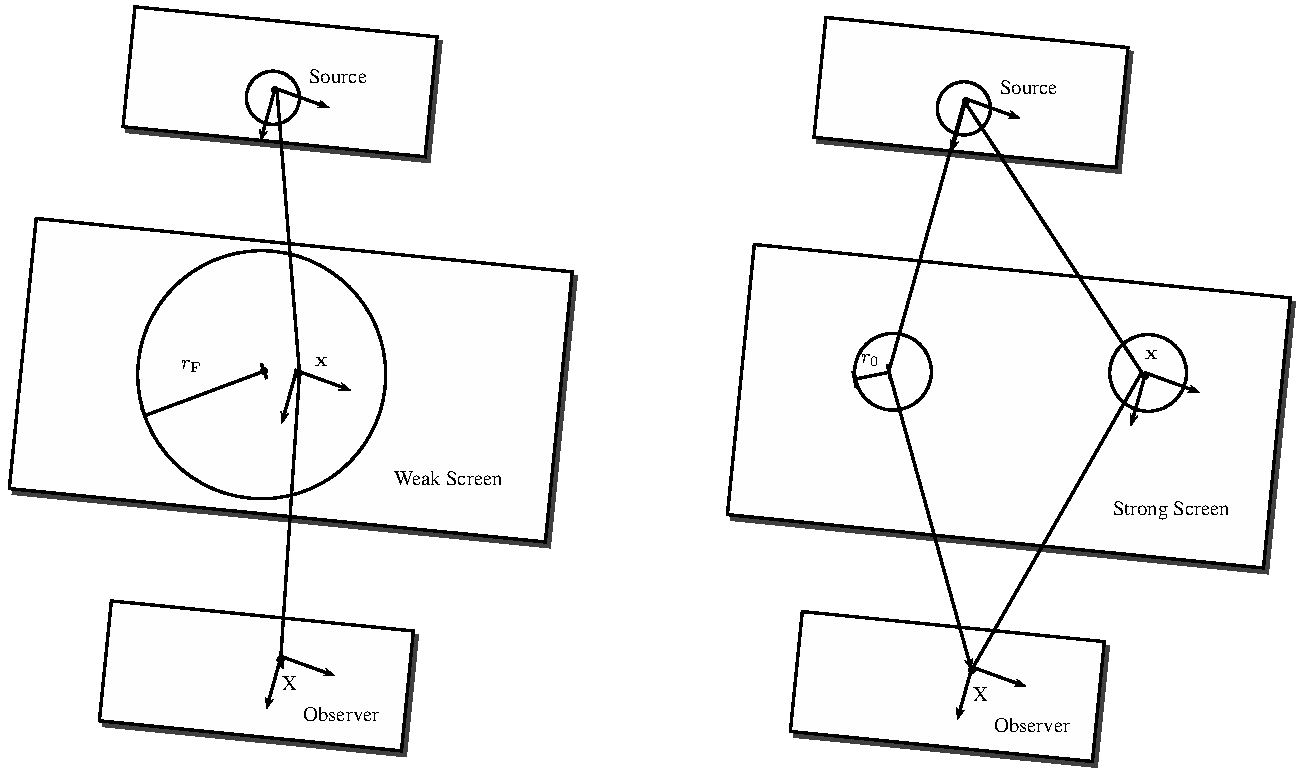
\includegraphics[width=1.\columnwidth]{Images/scatter.pdf}
\caption{Illustration depicting the basics of scattering in the weak (left) and strong (right) regimes. In the weak regime, the signal is coherently propagated over an area, $A_{\rm weak} \approx \pi r_{\rm F}^2$, whereas in the strong regime, coherent propagation is split over many areas, each of size $A_{strong} \approx \pi r_{\rm 0}^2$. \label{fig:scatter}
}
\end{center}
\end{figure*}

%frozen screen
To evolve the screen in time, we assume a frozen screen i.e. that the velocity of the individual turbulent eddies is dominated by the bulk motion of scattering medium \citep[e.g.][]{Lay_1997}. This allows us to treat the screen as frozen but advected over the observer by a constant motion. Hence time variability can be easily incorporated by the relative motion between source, scattering screen and observer.

\subsection{Interstellar medium scattering}\label{sec:ism_scat}
%PR 1 St 1 

%introduction and plan
Electron density inhomogeneities in the interstellar medium (ISM) plasma scatter the radio emission from the Galactic Centre. Radio interferometric observations of Sgr~A$^\star$ have characterised the basic properties of the intervening plasma matrial, however extensive developments in scattering theory and simulations have proved essential to the interpretation of more subtle scattering phenomena. This section begins with the earlier, longer wavelength VLBI results which studied the Gaussian blurring effect of the scattering of SgrA*; we then expand on the scattering theory introduced in Sec.~\ref{sec:basic_scat} to review the latest theoretical developments which explore the presence of scattering-induced substructure; finally we review recent observational results which account for scattering substructure in their data interpretation. 


%blurring
The dominant observational effect of this scattering scenario for $\lambda \gtrsim 1$~cm is to convolve the intrinsic source structure with an elliptical Gaussian. The size of the Guassian exhibits a $\lambda^2$ scaling dependence over several orders of magnitude \citep[Fig.~\ref{fig:scattering_law}][]{Backer_1978, Shen_2005, Bower_2006, Lu_2011},which is consistent with the wavelength dependence of the refractive index of a plasma. In order to determine the parameters of the scattering kernel, i.e. major axis, minor axis and position angle,  one has to observe at wavelengths where the angular size of scattering ellipse is much larger than the expected source size. A Very Long Baseline Array (VLBA) + Green Bank Telescope (GBT) campaign \cite{Bower_2006} estimated the size at $1.31 \times 0.64$~mas cm$^{-2}$, oriented $78^\circ$ east of north. 


%debluring,uncertainties of the extrapolation
An accurate extrapolation of scattering kernel to 1.3~mm is important for the EHT scattering-mitigation strategy \cite{Fish_2014} which aims to deblur the scattered image through a deconvolution procedure. However as this extrapolation is over at least an order of magnitude, any small systematic error in the original measurement can significantly effect the 1.3~mm extrapolated parameters. A recent review of VLBI observations of Sgr~A$^\star$ \cite{Psaltis_2015} has noted that there are significant inconsistencies between different measurements. The authors used a Bayesian methodology to re-analyse the datasets resulting in increased uncertainties as shown in table~\ref{tab:ism_gauss}. The minor axis has a much larger uncertainty than the major axis due to the limited north-south coverage of the VLBA array. 
%fig showing power laws of scattering and intrinsic source
\begin{figure*}
\begin{center}
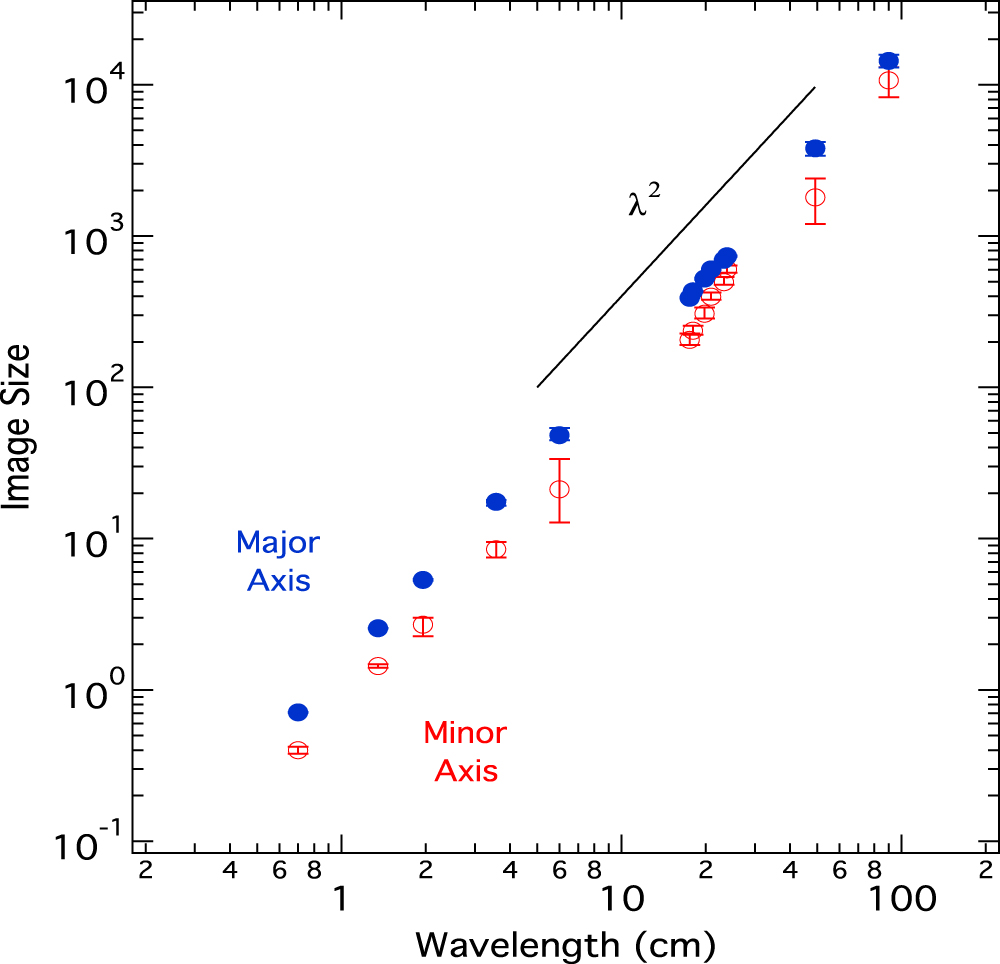
\includegraphics[width=0.6\columnwidth]{Images/scattering_law}
\caption{The $\lambda^2$ dependence of scattering kernel size is shown by the solid line. This has been derived from measurements made at $\lambda > 17$~cm \protect\cite{Bower_2006}. The dotted line shows the derived intrinsic source size which scales as $\lambda^{1.44}$. This was derived from measurements in the wavelength range, 2~cm~$< \lambda < 1.3$~mm \citep{Doeleman_2008}. The red circles show major-axis observed sizes of Sgr~A$^\star$  and the green points show the derived intrinsic major-axis size. This plot was reproduced from \protect\citet{Doeleman_2008}.\label{fig:scattering_law}
}
\end{center}
\end{figure*}
%table showing latest scattering kernel parameters
\begin{table}[]
\centering
\caption{A re-analysis of VLBI observations of Sgr~A$^\star$ by \citet{Psaltis_2015} has yielded revised estimates of the parameters associated with the Gaussian scattering kernel. Note that the position angle is measured East of North. \label{tab:ism_gauss}}
\begin{tabular}{l|ll}
\hline
major axis FWHM (mas/cm$^-2$)& 1.32 & 0.04 \\
minor axis FWHM (mas/cm$^-2$)& 0.82 & 0.21 \\
position angle ($^\circ$)& 77.8 & 9.7\\  
\hline
\end{tabular}
\end{table}


%theory - refractive scale and size of blurred image
The Gaussian blurring effect can explained by the simple scattering model introduced in  Sec.~\ref{sec:basic_scat}. Recall, that in the strong scattering regime light is propagated from coherent patches with linear size $\sim r_0$. Each patch will emit light coherently into a single-slit diffraction cone of angular size $\theta_{\rm scatt} \sim \lambda /r_0$. An observer will hence be illuminated by many patches spanning $\theta_{\rm scatt}$, yielding a blurred and broadened image, with projected size on the screen equal to the \emph{refractive scale} 
$$r_{\rm ref} = \theta_{\rm scatt} D_{\rm os} = r_{\rm F}^2/r_0.$$
$r_{\rm ref}$ is the third fundamental length scale in the strong scattering regime and is associated with the refractive timescale,
$$t_{\rm ref} = r_{\rm ref}/v.$$
%calculating r_0 given \theta_scatt 
We can calculate $r_0$ given the FWHM of $\theta_{\rm scatt}$ through the more precise relation
\begin{equation}\label{eq:theta_scatt}
 \theta_{\rm scatt} = \frac{2\sqrt{2\ln{2}}}{2\pi} \lambda / r_0 (M+1)
\end{equation} 
where $M = D_{\rm os}/R$ is the magnification and $R$ is the source-screen distance. The magnification factor is a correction to the model introduced in Sec.~\ref{sec:basic_scat} when $R \approx \infty$ no longer holds and should be used when calculating distances in the observer plane \citep*{Goodman_1989}.
%Locating the scattering screen Bower 2014
The location of the scattering medium was originally thought to be quite close to Sgr~A$^\star$. However, observations of a newly discovered pulsar, SGR~J1745-29, indicate that the scattering screen is located at a distance $D_{\rm os} = 5.8 \pm 0.3$~kpc, within the Scutum spiral arm. Using Eq.~\ref{eq:theta_scatt} and the parameters given in table \ref{tab:ism_gauss}, we find that the major axis of the coherence length at 1.3~mm, $r_0 \approx 3136.67$~km.


%shift to looking at refractive effects,theory, 3 regimes of scattering
As the VLBI moves to higher frequencies, focus has shifted away from the well-studied Gaussian convolution effect of ISM scattering and onto the presence of stochastic scattering-induced substructure. To understand this phenomenon, we must first develop the theory to be sensitivity to the averaging effects of the observation. 

Strong scattering can be further subdivided into \emph{snapshot}, \emph{average} and \emph{ensemble-average} regimes \citep*{Narayan_1989,Goodman_1989}. To understand the different regimes, remember that for each point on the source, the observer sees emission from coherent patches of area $\sim \pi r_0^2$ over an area $\sim \pi r_{\rm ref}^2$. The diffraction cones from each of the patches will interfere, resulting in a multi-slit \emph{diffractive scintillation} pattern. 

%snapshot regime
In the \emph{snapshot regime}, a compact source is observed with a narrow bandwidth and over a short time integration. This yields a single realisation of the diffractive scintillation pattern. By averaging over many snapshots, diffractive scintillation is quenched. This occurs if the source size $\theta_{\rm src}$ is much larger than the diffractive scale $\theta_{\rm src} \gg r_0/D_{\rm os}$; if the fractional bandwidth $\delta \nu/\nu$ is much larger than the decorrelation bandwidth $\delta \nu/\nu \gg \delta \nu_{\rm dc}/\nu \approx (r_0/r_{\rm F})^2$ \citep{Narayan_1992}; or if the integration time $t_{\rm int}$ is much larger the diffractive timescale $t_{\rm int} \gg t_{\rm 0} = r_0/v$, where $v$ is the relative velocity between screen, source and observer. This regime is hence only accessible through observations of compact objects like pulsars. On a side note, observations in this regime can be used to probe the source with angular resolution $\sim \lambda /r_{\rm ref}$ \citep[e.g.][]{Gwinn_2012}. This is because the scattering screen is essentially a lens of diameter $\approx r_{\rm ref}$.

%average regime 
In the \emph{average regime}, diffractive scintillation has been averaged over, however there still exists scintillation over scales comparable to the size of the scattered image of a point source $\sim r_{\rm ref}$, termed \emph{refractive scintillation}. Phase fluctuations on this scale acts like a weak lens to focus or defocus the $\lambda/ r_0$ scale diffraction cones in the direction of the observer. For a point source this would lead to weak flux variations in the total flux \citep{Narayan_1992}. We will show later that refractive scintillation leads to the presence of substructure for a resolved scatter-broadened source. In contrast to diffractive scintillation, refractive scintillation is much more difficult to average over. Typically the refractive time scale $t_{\rm ref} = r_{\rm ref}/v$ is on the order of weeks to months for scattering towards the Galactic Centre; the fractional decorrelation bandwidth is on the order of unity $\delta \nu_{\rm dc}/\nu \sim 1$; and the source has to be much larger than the image of a scattered point source $\theta_{\rm src} \gg \theta_{\rm scatt}$. 

%ensemble average
In the \emph{ensemble-average regime}, both diffractive and refractive scintillation have been averaged over. It is in this regime when  the scattering is equivalent to Gaussian convolution which is deterministic and not time variable. 


%approximation of the scattered image by Johnson 2015
A recent theoretical work \citep*{Johnson_2015a} has derived a useful approximation of the resolved scattered image $I_{\rm ss}$ in the average regime,
\begin{equation}\label{eq:scatterbrane}
I_{\rm ss}(\bm{x}) \approx I_{\rm src}\left(\bm{x} + r_{\rm F}^2 \nabla \phi(\bm{x})\right),
\end{equation}
where $\nabla$ is the directional derivative. Here we have used the same two-dimensional coordinate system, indexed by $\bm{x}$ to describe the source, screen and observer planes which are considered to be aligned along the vertical axis. The scattered image $I_{\rm ss}$ is approximated by a `reshuffling' of the source image $I_{\rm src}$. As $|\nabla\phi| \sim 1/r_0$, the magnitude of the translation of points on $I_{\rm src}$ $\sim r_{\rm ref} \sim 10\ \mu$-arcsec in the case of Sgr~A$^\star$. 

%Coherence of the phase slope 
Even though $\phi(\bm{x})$ is only coherent to $\sim r_{\rm 0}$, $\nabla \phi(\bm{x})$ remains spatially coherent over much larger scales. The autocovariance of phase derivative can be related to the structure function \citep*{Johnson_2015a}
\begin{equation} 
\langle [ \partial_x \phi(\bm{x_0})] [ \partial_x \phi(\bm{x_0}+\bm{x})] \rangle = \partial_x^2 D_\phi(\bm{x}).
\end{equation}


A generalised structure function \citep{Tatarskii_1971, Narayan_1989} is quadratic ($r^2$) at small scales ($r<< r_{\rm in}$), Kolmogorov in the range $r_{\rm in}<r<r_{\rm out}$ and constant for $r>r_{\rm out}$. Taking the simplifying case of $r_{\rm in} \gg r_0$ and $r_{\rm in}<r<r_{\rm out}$ $D_\phi$ becomes\citep{johnson_dissertation},
\begin{equation}
D_\phi = \frac{2}{\beta}\left( \frac{r_{\rm in}}{r_0}\right)^{2-\beta} \left( \frac{r}{r_0}\right)^\beta 
\end{equation}

Hence, $\partial_r^2 D_\phi(\bm{r}) \propto r^{\beta-2}$. Therefore in the Kolmogorov regime ($\beta = 5/3$), the coherence of image shift relative to the refractive scale $\propto (r/r_0)^{-1/3}$. Note that a large inner scale extends coherence of $\nabla\phi$, whereas as $r \to r_{\rm out}$ the coherence falls quickly. Therefore, even though $\phi(\bm{x})$ is only coherent to $\sim r_{\rm 0}$, $\nabla \phi(\bm{x})$ remains spatially coherent over much larger scales, leading to the presence of refractive substructure \citep*{Johnson_2015a}. 

%Observations of substructure
A recent observation of Sgr~A$^\star$ at 3.5~mm by the VLBA+LMT \citep[see Fig.~ref{fig:substructure2}][]{Ortiz_2016} has measured non-zero closure phases on its longest baselines. However it was also shown in the data anaylsis that the measured values are consistent with expectation refractive scintillation assuming a circular Gaussian source of FWHM~$=130\ \mu$-arcsec. Another observation at 1.3~cm shows flux modulation due to scattering substructure $\sim 10$~mJy \citep{Gwinn_2014} and other predictions for $\lambda = 1.3$~mm show $\sim 60$~mJy for long East-West baselines and $\sim 25$~mJy for long North-South baselines \citep*{Johnson_2015a}, assuming a Gaussian source of FWHM~$=40\ \mu$-arcsec.

\begin{figure*}
\begin{center}
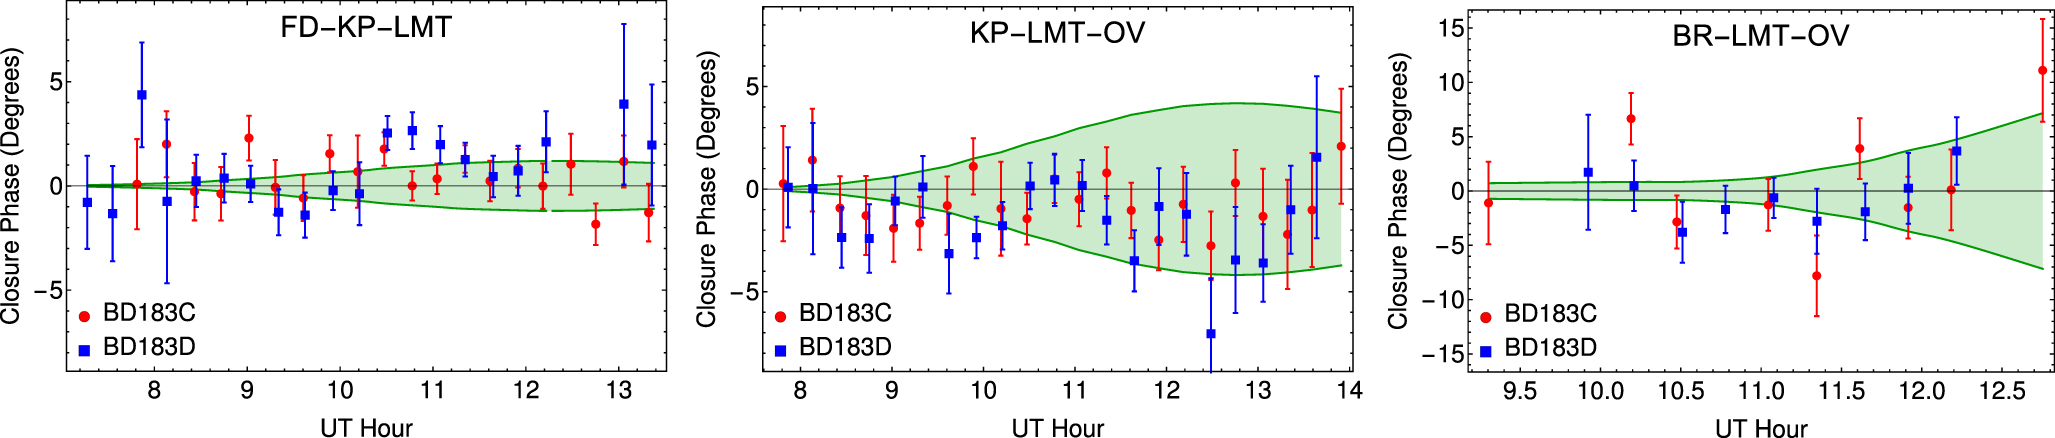
\includegraphics[width=\columnwidth]{Images/ism_cp}
\caption{Closure phases recorded in a VLBA + LMT observation of  Sgr~A$^\star$ at $\lambda = 3.5$~mm \protect\cite{Ortiz_2016}. The data points are shown as red circles and blue squares and are only distinguished by the calibrator used. The green envelopes show the $1\sigma$ closure phase prediction induced by scattering-induced substructure. Reproduced from \protect\citet{Ortiz_2016}. \label{fig:substructure2}
}
\end{center}
\end{figure*}


%Distinguishing intrinsic source structure and variability
Distinguishing intrinsic source and ISM substructure and variability is an interesting challenge. Observations at mm-wavelengths have revealed deviations from the $\lambda^2$ scattering scaling law, see Fig.~\ref{fig:scattering_law}. This is interpreted as due to the presence of intrinsic source structure and has been fitted with a power-law with an exponent of $1.34 \pm 0.01$ \cite{Lu_2011}. This has enabled the constraint of various theoretical models \cite{Bower_2006}, excluding advection-dominated accretion flows (ADAF) \cite{Narayan_1998} and Bondi-Hoyle accretion \cite{Melia_1994}. However observations extending over month timescales are required to properly sample the larger scale inhomogeneities and even with multiple epoch observations, it can be difficult to distinguish source and scattering characteristics \citep*{Macquart_2006}. The developments in scattering theory presented above provide a robust mechanism for quantifying refractive effects. This could allow a decoupling without sampling a refractive ensemble but significant assumptions are always made on the source model. 


\subsection{Troposphere}
%PR 1 St 1

%Introduction - Troposphere is a problem. Define troposphere. st 1
The coherence and intensity of millimetre wavelength electromagnetic waves are most severely deteriorated in the lowest atmospheric layer, the troposphere which extends up to an altitude of $7-10$~km above sea level and down to a temperature $T \sim 218$~K \citep{Thompson_2001}. The troposphere is composed of a number of different components including primary gases $\rm N_2$ and  $\rm O_2$, trace gases e.g. water vapour and ${\rm CO_2}$, as well as particulates of water droplets and dust. The rest of this section will explore the tropospheric corruption for the mm-VLBI case beginning with insights from the fundamentals of electromagnetic propagation, followed by a review of atmospheric corruptions in the sub-mm regime. We then firm up our theory with a discussion on atmospheric radiative transfer and atmospheric turbulence. 


\subsubsection{Propagation fundamentals}\label{sec:prop_fund}
%propagation fundamentals st 1
Consider a quasi-monochromatic wave passing through a linear medium,
\begin{equation}
E_\nu(x,t) = E_0 \exp^{i(kn_\nu x - 2\pi\nu t)},
\end{equation}		
where $k=2\pi \nu/c$ is the propagation constant in free space and $n= n_{\rm R} + j n_{\rm I}$ is the complex index of refraction. Note that we will occasionally omit the frequency dependence of $n$ and related quantities to simplify the notation. If $n_{\rm I}$ is nonzero, the electric flux $I$ will decay exponentially
\begin{equation}
I = EE^\ast = E_0^2 \exp(-\tau),
\end{equation}
where $\tau$ is called the opacity or optical depth and is related to the absorption coefficient, $d\tau = \kappa dx$ where $\kappa = 4\pi \nu n_I/c$. If $n_{\rm R} > 1 $ the phase velocity of light will decrease, $v_{\rm p} = c/n_{\rm R}$, which results in a time delay. The time delay due to the troposphere, $\tilde{t}$ and opacity $\tau$ can be calculated simultaneously,
\begin{equation}\label{timedelay}
\tilde{t} + i \tau /4\pi \nu =1/c \int_{path} d\bm{s}\  (n_\nu(\bm{s}) -1).
\end{equation}

%the relationship between delay-absorption-noise st 1
In the interferometric context opacity and time delay are often viewed independently. However, the electric field is real and causal which imposes restrictions on the complex refractive index. Specificially $n_{\rm R}$ and $n_{\rm I}$ contain the same information and can be interchanged via the Kramers-Kronig relations. 

Absorption is accompanied by emission and for a medium in local thermodynamic equilibrium, Kirchoff's law states that 
\begin{equation}\label{kirchoff}
\frac{\epsilon_\nu}{\kappa_\nu}=B_\nu(T),
\end{equation}
where $\epsilon_\nu = dI_\nu/dx$ is the emission coefficient and $B_\nu(T)$ is the Planck function. Hence the absorbing molecules are also emitters, increasing system noise. Therefore opacity, time delay and atmospheric noise are interrelated and should be simulated consistently. On a side note these relations allow for phase calibration using measurements of sky emission via Water Vapour Radiometry (WVR) \citep*[e.g.][]{Carilli_1999}.

\subsubsection{Atmospheric corruptions in the (sub-)mm regime}
%st 1
%Absorption in the GHz regime st 1
An analysis of the absorption spectrum in the GHz range (Fig.~\ref{fig:absorption}), shows that it is dominated by transitions of $\rm H_2O$ and $\rm O_2$ as well as a pseudo-continuum opacity which increases with frequency. The pseudo-continuum opacity is due to the cumulative effect of the far wings of a multitude of broadened water vapour lines above 1~THz \citep{Carilli_1999}. At 230~GHz the absorption is typically $5-10$\% at the best sites, during good weather. 

%Fig Absorption spectrum in the GHz st 1
\begin{figure*}
\begin{center}
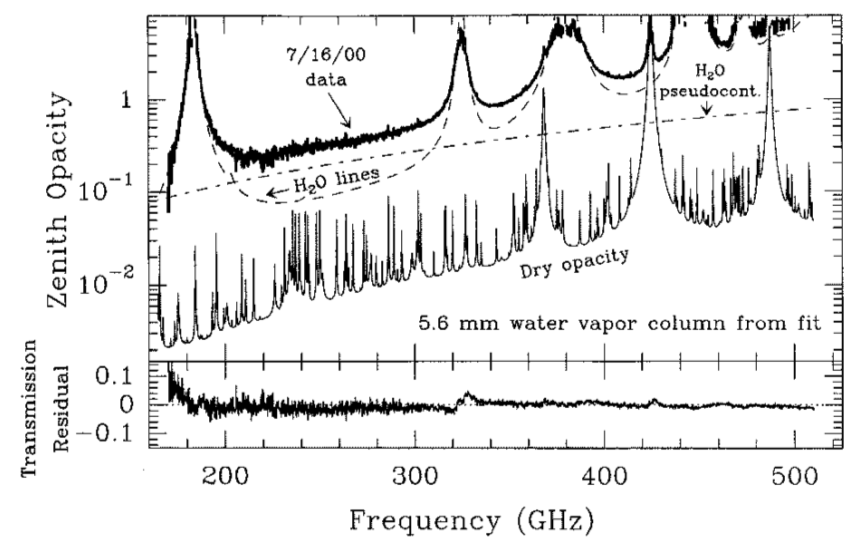
\includegraphics[width=\columnwidth]{Images/absorption}
\caption{Recorded zenith absorption spectrum in the $160-520$~GHz range, taken on Mauna Kea at an altitude of $\approx 4000$~m. The data has been fit to a sum of $\rm H_20$ lines, an $\rm H_20$ pseudo-continuum and dry absorption lines. The model has been generated using the \textsc{atm} code (see section~\ref{sec:atm_theory}), with the bottom panel showing the residuals. Here `dry' refers to all atmospheric constituents except $\rm H_20$. Reproduced from \citet{Pardo_2001} \label{fig:absorption}
}
\end{center}
\end{figure*}

%Phase variability in the GHz st 1
In contrast to the dry atmospheric components, water vapour mixes poorly and its time-variable spatial distribution induces rapid fluctuations in the time delays $\tilde{t}$ above each station. The phase error for a baseline (1,2) where antenna 1 is the reference will be
\begin{equation}\label{eq:phase_ref}
\delta \phi(t, \nu) = 2\pi/\nu(\tilde{t}_2(t, \nu) - \tilde{t}_1(t, \nu)).
\end{equation}
The water vapour column volume is measured as the depth of the column when converted to the liquid phase and is referred to as the precipitable water vapour (PWV). PWV is directly proportional to the time delay and hence the phase delay, 
\begin{equation}
\delta\phi \approx \frac{12.6\pi}{\lambda} \times w, 
\end{equation}\label{eq:phi-pwv}

\noindent where $w$ is the depth of the PWV column \citep*{Carilli_1999} and an atmospheric temperature $T=270$~K has been assumed. This relationship between phase and water vapour content has been experimentally verified \citep{hogg_1981}. At 230~GHz, the change in PWV needed to offset the phase by 1~rad is $\Delta w\approx0.03$~mm. 

This sensitive dependence of phase coherence on atmospheric stability is aggravated by three factors. First antenna elevation angles are typically fairly low for EHT observations which increases the atmospheric path length. Second as stations are far apart the atmospheric variations are uncorrelated between stations, this increases visibility decoherence as atmospheric variations appearing in both terms of equation~\ref{eq:phase_ref} fall away. Third, observing with a sparse VLBI array means that there is less redundancy for calibration and so it is more difficult to separate source from atmospheric variations.


\subsubsection{Radiative transfer}\label{sec:atm_theory}
%St 1

%Radiative transfer, how solving it will give observables in a self-consistent manner st 1
The problem of radiative transfer through a static atmosphere is well described and implemented by the Atmospheric Transmission at Microwaves (\textsc{atm}) software \citep{Pardo_2001}. \textsc{atm} has been incorporated into \textsc{MeqSilhouette} to provide a fast and sophisticated procedure to calculate average opacities, sky brightness temperatures and time delays. Here we provide a brief summary of the theory underpinning the package but refer the reader to \citet{Pardo_2001} for more detail. \textsc{atm} is commonly used in the Atacama Large Millimeter Array (ALMA) community \citep{Curtis_2009,Nikolic_2013} and has been tested with atmospheric transmission spectra taken on Mauna Kea \citep{Serabyn_1998}.

%Radiative transfer st 1
We start from the unpolarised radiative transfer equation, which is unidirectional in the absence of scattering,
\begin{equation}\label{eq:rad_trans}
\frac{dI_\nu (s) }{ds} = \epsilon_\nu(s) -\kappa_\nu(s)  I_\nu (s),
\end{equation}
where $s$ is the coordinate along the signal path through the atmosphere. We assume local thermodynamic equilibrium (LTE) which should hold as the collisional timescale is much smaller than the time for spontaneous emission for all but the highest part of the atmosphere. Applying equation~\ref{kirchoff}, multiplying by $\exp(-\tau_\nu)$ and integrating from the top of the atmosphere ($s=0$) yields, 
\begin{equation}\label{eq:rad_trans2}
I_\nu(s) = I_\nu(0) e^{-\tau_\nu (0,s) }+ \int_0^s B_\nu(s')e^{-\tau_\nu (s',s) }\kappa_\nu(s')ds',
\end{equation}
where  $s'$ is a dummy variable in the same direction as $s$ and $\tau_\nu (0,s) = \int_0^{s} k_\nu(s')ds'$. $I_\nu(0)$ is normally taken as the radiance from the cosmic background.
To calculate the $I_\nu(s)$, $\tau(s)$ and complete the above integral, requires $\kappa_\nu$ as a function of altitude and frequency. The time delay $\tilde{t}$ can be calculated from $\tau$ using the Kramers-Kronig relations. 


%deriving the absorption coefficient st 1
A general equation to determine the absorption coefficient for a transition between a lower $l$ and upper $u$ states is given in the original paper. Here we merely point out that it should be proportional to the energy of the photon, $h\nu_{l \to u}$, the transition probability or Einstein coefficient, $ B_{l \to u}$, the line-shape, $f(\nu,\nu_{l \to u})$ and the number densities $N$ of electronic populations. Line profiles which describe pressure broadening (perturbations to the Hamiltonian due to the presence of nearby molecules) and Doppler broadening are used. The condition of detailed balance further requires that decays from the upper state are included yielding, $g_u B_{u \to l} =g_l B_{l \to u}$, where $g$ is the degeneracy of the electronic state. Putting this together we find,

\begin{equation}
\kappa(\nu) _{l \to u}  \propto  h\nu   B_{l \to u}  \left(\frac{N_l}{g_l}  -  \frac{N_u}{g_u} \right) f(\nu,\nu_{l \to u}),
\end{equation}

\noindent where the Einstein coefficients are calculated from the inner product of the initial and final states with the dipole transition operator,\begin{equation}\label{coefficient}
B_{l \to u} = \frac{2\pi}{3\hbar^2} |<u|\mu|l>|^2,
\end{equation}
where $|u>$, $|l>$,$|\mu>$ are the wavefunctions of upper and lower states and the dipole transition operator respectively. The number densities of the two states, $N_u$ and $N_l$ in local thermodynamic equilibrium (LTE) are simply related to the local number density and temperature via Boltzmann statistics. 
\begin{equation}
\frac{N_n}{N} = g_n \frac {\exp{-\frac{E_n}{kT}}}{Q}
\end{equation}
where Q is the partition function. $Q = \sum_i g_i  \exp{-E_n/kT}$. 
%inner product st 1
Transition lines at radio wavelengths result from rotational state transitions. To calculate the inner product given in equation~\ref{coefficient}, Operators which describe linearly symmetric rotors (e.g. ${\rm O_2}$, ${\rm CO}$) and asymetric rotors are used. The asymetric rotations are decomposed into three principal rotation axes with differing rotational constants governing each axis. Rotational constants were measured by the authors as well as drawn from a variety of literature. Partition functions and transition probability are calculated using approximations taken from the literature.
 

%lineshapes and pseudocontina st 1 
Far wing broadening of ${\rm H_2O}$ lines~$> 1.2$ THz extends to lower frequencies and is not completely represented by the line-shape used. This is believed to be due to self-self collisions of water molecules. Additionally there are terms from the dry atmosphere related to transient dipoles and Debye absorption which are not represented in the line-shape. To correct for these effects, two pseudocontina are used. These are modelled as a power law dependence on frequency, temperature and the molecular densities. 


\subsubsection{Turbulent phase fluctuations}\label{sec:turb_theory}
%St 1

%phase fluctuations as a calibration problem st 1
Visibility phase instability  $\delta \phi(t)$ due to tropospheric turbulence is a fundamental limitation to producing high fidelity, science-quality maps with a mm-VLBI array \citep{Thompson_2001}. The coherence time-scale is typically too rapid ($\lesssim10$~s) for fast switching calibration, so other calibration procedures (e.g. water vapour radiometry, paired antennas, and/or self-calibration) must be performed. Self-calibration is the most commonly used but is limited by the integration time needed to obtain adequate SNR to fringe fit. Phase decoherence often leads to the use of closure quantities to perform model fitting \citep{Doeleman_2001,Bower_2004, Shen_2005}, and causes a decrease in measured flux due to incoherent complex averaging.
%plan
In the section we will review and develop the weak scattering theory introduced earlier which will culminate in a formulation for the simulation of tropospheric phase turbulence seen by a mm-VLBI array. How this formulation is implemented and fits into the broader atmospheric simulation framework will be discussed in section~\ref{sec:trop_imp}. 


%Following from scattering intro, weak scattering model setup st 1
Following from section~\ref{sec:basic_scat}, we model the statistics of $\delta \phi(t)$ with a thin, frozen, Kolomogorov-turbulent phase screen moving with a bulk velocity, $v$. 
%Discussion on thickness of turbulent layer st3
However, the turbulent layer has a definite width $\Delta h$ and both Kolmorogov theory and measurement \citep[Fig.~\ref{fig:screentransition},][]{Coulman_1985, Treuhaft_1987, Carilli_1997} show that this brings in a new regime
\begin{equation}
 \beta = \left\{
 \begin{array}{rl}
 5/3 & \text{if } r < \Delta h,\\
2/3 & \text{if } r > \Delta h,\\
0 & \text{if } r > r_{\rm out}.
 \end{array}
\right\}
\end{equation}

In Fig.~\ref{fig:screentransition} we can see estimations of $\Delta h \approx 1$~km and $r_{\rm out} \approx 6$~km. We will show later that even though we are working with a VLBI array, our implementation falls in into the $r \ll \Delta h$ regime.


%Fig. Phase variability carilli_1997 st 1
\begin{figure*}
\begin{center}
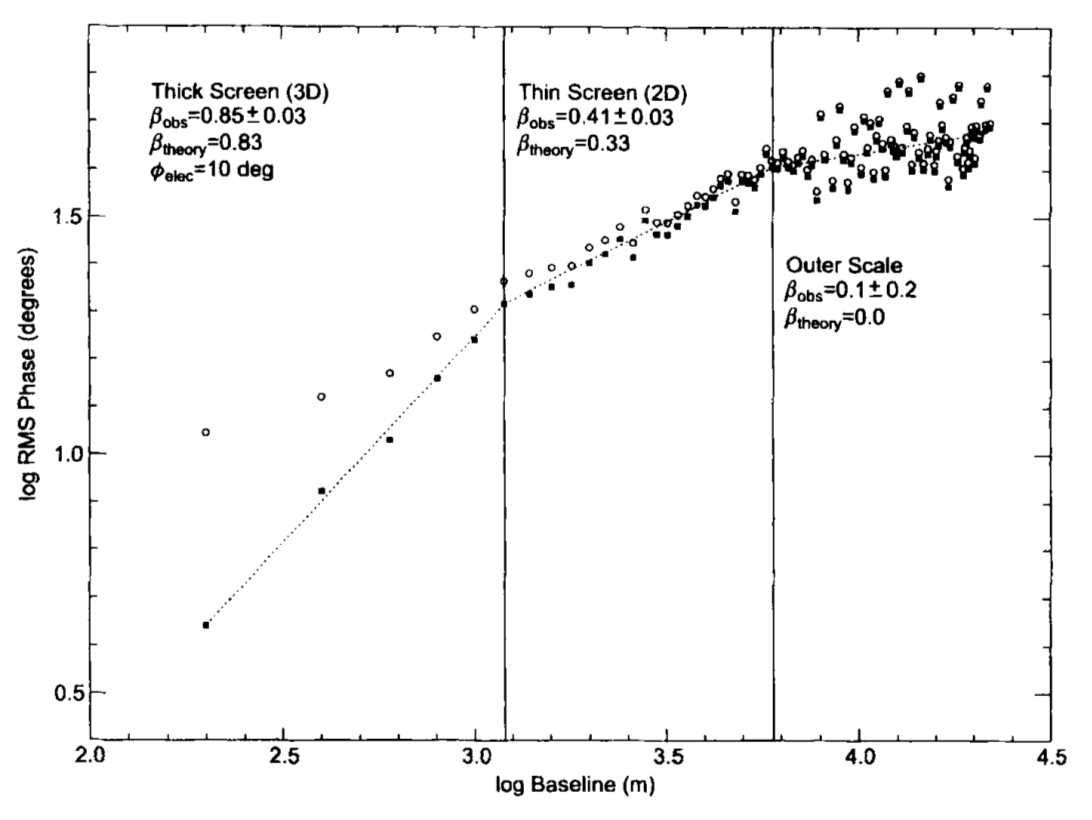
\includegraphics[width=\columnwidth]{Images/screentransition}
\caption{A log-log plot of RMS visibility phase versus baseline length for an observation of 1~Jy source 0748~+~240 with VLA at 22~GHz over a 90~min duration. The open circles show RMS phase as measured whereas the solid squares show the same values with a constant thermal noise contribution of $10^\circ$ subtracted in quadrature. Note that the measured and theoretical Kolmogorov turbulent exponent $\beta$ changes with distance on the phase screen as the viewing configuration transitions from a thick screen ($\beta_{\rm theory} = 5/3$) to a thin screen ($\beta_{\rm theory} = 2/3$) at $r \approx 1$~km and from a thin screen to completely uncorrelated regime ($\beta = 0$) beyond the outer scale at $r \approx 6$~km. Although these regimes appear distinct, there is continous variation between them. Reproduced from \citet*{Carilli_1997} \label{fig:screentransition}
}
\end{center}
\end{figure*}

 %weak scattering model setup st 1
 We set the height $h$ of the screen at the water vapour scale height of 2~km above ground.At $1.3$~mm, the Fresnel scale is $r_F \approx 0.45$~m and experiments show annual variations of $r_0 \sim 50 - 500$~m above Mauna Kea \citep{Masson_1994} and $r_0 \sim 90 - 700$~m above Chajnantor \citep*{Radford_1998}, where both sites are considered to have excellent atmospheric conditions for millimetre astronomy. As $r_F < r_0$, this is an example of weak scattering. 



%simplifying the scattering model st 1
The required field-of-view (FoV) of a global mm-VLBI array is typically FoV~$< 1$~mas or ~$\sim10~\mu$m at a height of 2~km, which is roughly 7-8 orders of magnitude smaller than the tropospheric coherence length. The tropospheric corruption can therefore be considered constant across the FoV and, from the perspective of the Measurement Equation, modeled as a diagonal Jones matrix per time and frequency interval. As VLBI baselines are much longer than the coherence length, $|\bm{b}| \ge 1000$~km~$\gg \rm r_0$, the phase screen at each site must be simulated independently. This assumption only holds for VLBI baselines and the framework needs to be extended to simulate the effects of turbulence on individual phased arrays stations (e.g. SMA) and short ($<10$~km) baselines (e.g. JCMT - SMA). 

%structure function formulation st 1
Our aim then is to produce a phase error time sequence $\left\{\delta \phi(t_i)\right\}$ for each station which is added to the visibility phase. We invoke the frozen screen assumption and write the structure function as a function of time, ${D (t) =  D(r)|_{r=vt}}$. The temporal structure function $D(t)$ provides an efficient route to sample the variability of the troposphere at the typical integration time of the dataset, $t_{\rm int} \sim 1$~sec. 

The temporal variance of the phase is a function of the temporal structure function, and accounting for time integration yields \citep*[see][B3]{Treuhaft_1987} 

\begin{equation}
\sigma^2_{\phi}(t_{\rm int}) = (1/t_{\rm int})^2 \int_{0}^{t_{\rm int}} (t_{\rm int}-t) D_{\phi}(t) dt.
\end{equation}

Assuming power-law turbulence and integrating yields, 

\begin{equation}\label{eq:turb_final}
\sigma^2_\phi (t_{\rm int})=\left[\frac{1}{\sin\theta(\beta^2 +3\beta +2)}\right]\left(\frac{t_{\rm int}}{t_0}\right)^{\beta},
\end{equation}


\noindent where $t_0 = r_0/v$ is the coherence time when observing at zenith and $1/\sin\theta$ is the approximate airmass which arises as $D_\phi \propto w$. As $r \ll \Delta h$, where $\Delta h$ is the thickness of the turbulent layer, an thin screen exponent of $\beta = 5/3$ is justified \citep*{Treuhaft_1987}. The phase error time-series takes the form of a Gaussian random walk per antenna. At mm-wavelengths, the spectrum of water vapour is non-dispersive up to a few percent \citep{Curtis_2009} and so we can assume a simple linear scaling across the bandwidth.






%A comparison to the phase screen approach st 1
Phase fluctuations $\delta\phi(t)$ can also be simulated by taking the inverse Fourier transform of the spatial phase power spectrum. However this approach is much more computationally expensive, e.g. for an observation length $t_{\rm obs}$ involving $N_{\rm ant}=8$ independent antennae with dish radii $r_{\rm dish}=15$~m, wind speed $v=10$~m\,s$^{-1}$ and pixel size equal to $r_{\rm F}$, the number of pixels $N_{\rm pix} \approx N_{\rm ant} t_{\rm obs} r_{\rm dish}^2/(v r_{\rm F}^3)  \sim 10^8$. Additionally, due to fractal nature of ideal Kolmogorov turbulence, the power spectrum becomes unbounded as the wavenumber approaches zero which makes it difficult to determine the sampling interval of the spatial power spectrum \citep{Lane_1992}.


\subsection{Instrumental}

%plan
All instruments suffer from both systematic and stochastic errors, the characterisation of which are essential to high precision measurement. In this section we explore thermal noise (stochastic) and antenna pointing errors (systematic). 
%completeness and classes of corruptions
While there are many additional potential sources of error (e.g. clock errors, bandpass, polarisation leakage, phasing errors, quantisation, correlator model, etc.). The point here is to demonstrate the mm-VLBI framework that enables more sophisticated interferometric simulations. The Measurement Equation formalism, enables any arbitrary linear error to be incorporated as a Jones Matrix e.g. a bandpass error would be a frequency-dependent diagonal Jones matrix.

\subsubsection{Thermal Noise}
%Pr 1 St 1


%Mild derivation of the thermal noise equation.
The level of thermal noise of measurement defines the absolute limit on the sensitivity of the interferometer to detect a source and also to distinguish fine source characteristics. Closure quantities are especially prone to high levels of thermal as several visibilities are multiplied. A derivation of the thermal noise of an interferometer can be made through derivation of the thermal noise of an antenna and then correlating the result \citep*{Wrobel_1999}. The RMS thermal noise of an interferometer $\{i,j\}$ over a bandwidth $\Delta \nu$ and an integration time is given by 

\begin{equation}
 \Delta S_{\rm ij} = \frac{1}{\eta_{\rm s}}\sqrt{\frac{SEFD_{\rm i}\ SEFD_{\rm j}}{2 \Delta \nu t_{\rm int}}},  
\end{equation}
where $\eta_{\rm s}$ is the system efficiency and $2 \Delta \nu t_{\rm int}$ is the number of independent samples. The $SEFD$ is a measure of the sensitivity of an antenna, accounting for the effiency, collecting area and thermal noise and is defined as the flux density of a source with the same power,
\begin{equation}
 SEFD = 2 k_{\rm B} T_{\rm sys} / (\eta_{\rm a} A),
\end{equation}
where $A$ is the antenna area, $\eta_{\rm a}$ is the antenna efficiency, $T_{\rm sys}$ is the system temperature and the factor $\frac{1}{2}$ accounts for only sampling 1 polarisation.


% Link to RIME -> additive matrix
As the RIME was formulated for a thermal noise-free measurement, we do not apply this corruption as a multiplicative matrix but rather an additive matrix,
\begin{equation}\label{eq:noise_matrix}
\bm{V}_{pq} = \bm G_p \bm{X}_{pq} \bm G_q^H + \bm N_{pq},
\end{equation}
where each component of $N_{pq} \sim (0, \Delta S_{\rm ij}^2)$.


\subsubsection{Antenna Pointing}
%Pr 1 St 1
%Intro
All antennas suffer pointing errors to some degree due to a variety of factors including dish flexure due to gravity, wind and thermal loading, as well as drive mechanics. This corresponds to an offset primary beam, which should only translate to minor amplitude errors if the pointing error $\theta_{\rm PE}$ is significantly smaller than the primary beam (i.e. $\theta_{\rm PE} \ll \theta_{\rm PB}$). In the Measurement Equation formalism, this offset can be represented by a modified (shifted) primary beam pattern in the {\bf \it E}-Jones term 
\begin{equation}
{\bf E}_p(l,m) = {\bf E}(l_0 + \delta l_p, m_0 + \delta m_p),
\end{equation}
where $\delta l_p, \delta m_p$ correspond to the directional cosine offsets.
%Motivation, why this could be a problem for mm observations
This could be a problem for millimetre observations as the primary beam is significant, e.g. for a 30~m dish at 1.3~mm, $\theta_{\rm PB} \sim 10$~arcsec, compared to the$\theta_{\rm PE} \sim 1$~arcsec.

% Different categories of pointing error i.e. tracking vs slew

We identify two main classes of pointing error. Firstly an antenna tracking a source will suffer a slow, continuous time-variable pointing error associated with the tracking error $\sigma_{\rm track}$. Physically this could be attributed to changes in wind, thermal and gravitational loading which all change with telescope pointing direction and over the course of a typical few hour observation. Using the MeqTrees software package, such behaviour has been demonstrated to occur with the Westerbork Synthesis Radio Telescope (WSRT, \cite{Smirnov_2011c})\footnote{See also https://indico.skatelescope.org/event/\\171/session/9/contribution/20}.


Secondly, whilst a stationary phase centre is tracked, the pointing error should evolve slowly and smoothly, however, in mm-VLBI observations the phase centre is often shifted to another source/calibrator. This would cause the pointing error to change abruptly, with an absolute pointing error $\sim \sigma_{\rm abs}$. Source/calibrator change is scheduled every 5-10 minutes in a typical millimetre observation. The point is that even though EHT will be able to determine the pointing offset when observing a calibrator with well known structure, when the antennas slew back to a source (e.g. Sgr~A$^\star$) with less certain or variable source structure, the pointing error could change significantly. This is exacerbated by the scarcity of mm-wavelength calibrators, which are often widely separated from the source.

%\chapter{Software implementation}

\section{Design objectives}
%Pr 1 St 1
%broad objectives
Our primary aim is to test and research mm-VLBI calibration, imaging and parameter estimation algorithms/strategies through the construction of a synthetic data simulation framework. To address the many questions within the wide scope of this objective, one must be able to setup and run a diversity of experiments within the simulation framework. This places definite constraints on the software architechure. In particular, the framework should 


%specific objectives
\begin{itemize}
%framework for consistent implementation of the necessary signal corruptions  
 \item enable the implementation of all relevant classes of signal corruption within a formalism which ensures consistency with the causal signal transmission chain,
 %grmhd input
 \item be compatible with time-variable GRMHD source models which are to be used as inputs,
 %modularise - extendable
 \item be organised in modularised structure so that it is flexible, extendable and could be incorporated by other interferometric algorithms e.g. a calibration or a parameter estimation algorithm,
  %modularise - diverse experiments
 \item The modular structure should also enable the construction and execution of arbitrary observations.
\end{itemize}

\section{Architechure and Workflow}
%Pr 1 st 2
%Intro and plan, How to meet objectives %st 1
In this section, we will review how the architechural design and workflow of the simulator architechure has been designed to meet the above objectives. To fulfill the first objective, we try to cast signal corruptions in the RIME formalism (see section~\ref{sec:RIME}), and where this is not possible, to fit those particular signal corruptions into the casually correct position in the signal transmission chain, with proper consider given to non-communitivity of elements in the signal transmission path. The implementation of each signal corruption is described in the following subsections. The remaining objectives fall into the realm of software design and will be discussed in this subsection. 


%Language and data format choice
%st : fine + contained %st 1
We have chosen to write the high level simulation code using the \textsc{Python} language. \textsc{Python} is a general purpose language, is geared towards readability, and is well supported by a comprehensive library and wide user base (including astronomers). Specifically \textsc{Python} interfaces well with a modern interferometric toolbox, {\sc MeqTrees}, as well as our data formats of choice: {\sc fits} for image cubes and the {\sc measurement set}\footnote{https://casa.nrao.edu/Memos/229.html} {\sc ms} for visibilities. Although the higher level functionality is written in \textsc{Python}, the bulk of the computational load ({\sc ms} and visibility generation) is called through the faster {\sc C++} language. 
We use {\sc ms} as our data format as it is directly accessible via the {\sc pyrap} library and is the data format used by {\sc MeqTrees} which performs the visibility generation and pointing error simulation. Although in the mm-VLBI subfield other data formats are currently still more popular than the {\sc ms}, i.e. {\sc UVFITS} or {\sc IOFITS}, with the completion of ALMA, the MS format should become the next modern data format and already is used at the Joint Institute for VLBI in Europe (JIVE). 


%Highest level architechure : Distinction between framework and driver and how they link %st 1
To create a flexible and modular structure necessary to be able to run a diversity of experiments, the software implementation is divided into 2 components:
\begin{itemize}
 \item an object-oriented framework into which is programmed the logic of each individual step in the signal propagation chain,
 \item a driver script which initialises the most abstract class in the framework with the required inputs and determines the signal propagation chain relevant to that particular pipeline.
\end{itemize}
The conceptual flow diagram of one realisation of a {\sc MeqSilhouette} simulation pipeline is shown in Fig.~\ref{flow}. To emphasise, the framework is not restricted to this sequence of operations, allowing the exact pipeline to be quite general. This flexibility is made possible through the use of \emph{Object-Orientation}, which will be elaborated on later. 


%Inputs %st 1
All inputs to the simulator are specified by a configuration file, containing a dictionary, which is the sole input to the driver script. This dictionary contains everything needed by the pipeline to determine the particular observation configuration (frequency, bandwidth, start time, etc), which signal corruption implementation should be employed and where the sky model and antenna table are located in the filesystem. Antenna table is in the CASA format, and can readily be created or altered using the {\sc pyrap} library using the station coordinates. The primary accepted sky model is a time-ordered list of {\sc fits} images, where each image represents the source total intensity over a time interval $\Delta t_{\rm src} = t_{\rm obs}/N_{\rm src}$, where $t_{\rm obs}$ is the observation length and $N_{\rm src}$ is the number of source images. Currently the pipeline only supports total intensity and the conversion of the pipeline to support full stokes is discussed in section~\ref{sec:discussion}. A variation of the pipeline has also been written which uses a parametric source model consisting of Gaussians or point sources as the sky model. This functionality was needed for the simulation of pointing errors as the {\sc MeqTrees} beams model does not support the {\sc fits} sky model.


%Outputs and Data products %st 1
The primary outputs of the pipeline are an interferometric dataset in MS format along with the closure phases (including uncertainties) and a dirty and/or deconvolved image. The modular structure of the pipeline allows for additional imaging and deconvolution algorithms to be easily appended to the final data processing steps. Noting that there are other data formats widely used in mm-VLBI, we make use of the {\sc casa} task for conversion to {\sc uvfits}. As the pipeline is easily flexible other data products can be easily produced as needed e.g. polarisation ratios or time-frequency averaged data.


%Overview of the workflow

%workflow fig : example of a pipeline %st 1

\begin{figure*}
\begin{center}
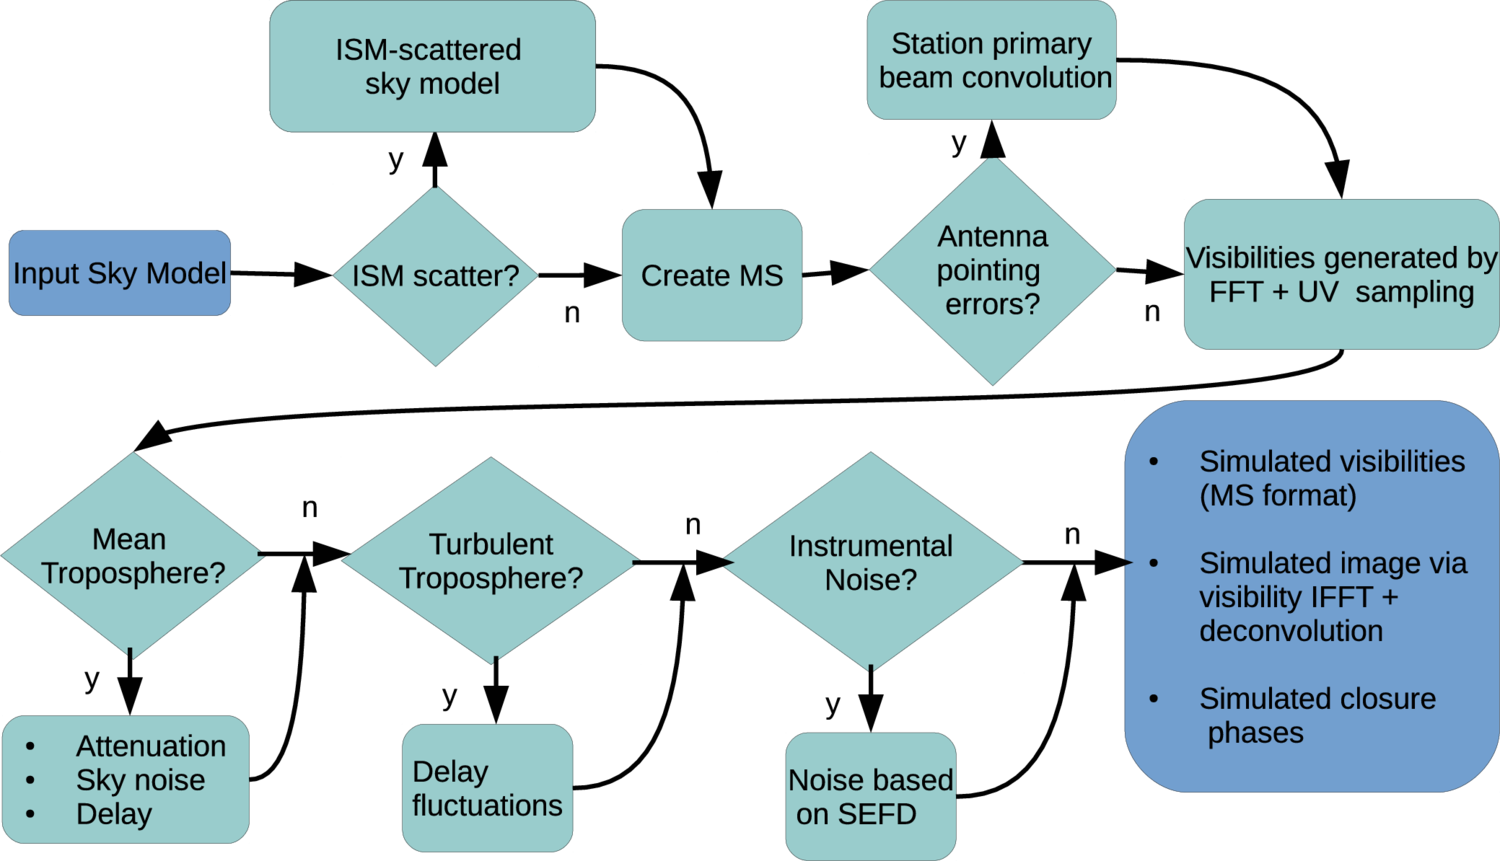
\includegraphics[width=\columnwidth]{Images/flow_full}
\caption{Flow diagram showing basic sequence of a \textsc{MeqSilhouette} simulation pipeline. The specific sequence is determined by the driver script whereas the logic of each step is contained in an object-oriented framework. The details of the station information, observation strategy, tropospheric and ISM conditions are specified in a user-defined input configuration file. The pipeline is extendable, allowing any additional, arbitrary Jones matrices to be incorporated. \label{flow}%
}
\end{center}
\end{figure*}

%Framework - details
%ms creation 
An important step to reproduce realistic observations is to be able create a comprehensive MS which can handle arbitrary scans lengths and start times as well as arbitrary frequency channelisation and bandwidth. This is performed using the {\sc simms}\footnote{https://github.com/radio-astro/simms} tool. {\sc simms} provides an easy to use interface to construct general MS, given an appropriate antenna table. The call is {\sc simms} is located within the driver script. 

% Calculation and & back end & object orientation
%SimpleMS
In order to make the framework as clean and  modular as possible we have made extensive use of object orientation. The first major class, \emph{SimpleMS}, was intended to abstract and modularise the MS and MS-only derived attributes (e.g. visibility data and station positions) and methods (e.g. functions to calculate station elevations and closure phases) as well as expose these attributes and methods more efficiently than following {\sc pyrap} procedures which become verbose when used frequently.

%TropMS
The second MS-related class, \emph{TropMS}, handles the calculations relevant to tropospheric and thermal noise corruptions. This class is a child of {\it SimpleMS} and is initialised with weather and station information. Note that a child contains all the methods and attributes of its parent. This allows the tropospheric corruption implementation to use, whilst being separated from, the core MS functionality. The details of the tropospheric corruption is provided in subsection\ref{sec:atm_imp}. 

%SimCoordinator
The third MS-related class is the \emph{SimCoordinator}, and it is a child of the {\it TropMS} class. {\it SimCoordinator} is designed to make arbitrary simulations easy and efficient to construct and execute on a high level. It is the only MS class directly initialised in the driver script and hence the low level functionality and attributes of its parents are abstracted from the user. In addition to inherited functionality, {\it SimCoordinator} can call the ISM-scattering task (see subsection~\ref{sec:ism_imp}), and {\sc MeqTrees} functionality. of visibilities and simulation of antenna pointing errors using the {\sc MeqTrees : turbo-sim} task, where the visibilities are calculated through evaluation of the Fourier Transform at each UVW coordinate in the dataset, the time and frequency resolution of which is specified by the user.
 

\subsection{ISM scattering}\label{sec:ism_imp}
%Pr 1 St 2

%Link back to theory
As described in section~\ref{sec:ism}, ISM scattering towards Sgr~A$^\star$ falls into the \emph{average regime}, wherein diffractive scintillation is averaged out but refractive scintillation is still present. As mm-VLBI observations can resolve the scatter-broadened image of Sgr~A$^\star$, an implementation of scattering is needed which approximates the subtle changes in its extended source structure. Such an approximation has been implemented in the \textsc{Python}-based \textsc{Scatterbrane}\footnote{http://krosenfeld.github.io/scatterbrane} package, and is based on \citet*{Johnson_2015a}. The algorithm generates a phase screen based on the two dimensional spatial power spectrum  \citep*[see][Appendix C]{Johnson_2015a} which incorporates inner and outer turbulent lengths scales and then implements \ref{eq:scatterbrane} using an interpolation function modified by the phase screen.


%Inputs & generality of scatterbrane
{\sc ScatterBrane} allows variation in all parameters associated with the scattering screen which is essential as aspects of the scattering towards the galactic centre is still unconstrained. 

%Within the power spectrum $r_0$, $r_{\rm in}$, $r_{\rm out}$, $D_{\rm os}$, $R$, screen resolution, The number of pixels on the screen, anisotropy of the scattering kernel, the turbulent exponent ,wavelength, accomadation of variability


%Integration of Scatterbrane
We include the {\sc ScatterBrane} software, which has already yielded important context for mm-VLBI observations towards Sgr~A$^\star$ \citep[e.g.][]{2016arXiv160106571O}, within the {\sc MeqSilhouette} framework. Our ISM module interfaces the \textsc{Scatterbrane} code within an interferometric simulation pipeline. This module enables simultaneous use of time-variable ISM scattering and time-variable intrinsic source structure within a single framework. The user is able to select a range of options relating to the time-resolution and epoch interpolation/averaging of both. By default, if the time resolution chosen to sample the source variability $\Delta t_{\rm src}$ and screen variability $\Delta t_{\rm ism}$ are unequal, we set  
\begin{itemize}
 \setlength\itemsep{1em}
\item $\Delta t_{\rm ism}=\Delta t_{\rm src}$ \qquad \qquad if \qquad  $\Delta t_{\rm src} < \Delta t_{\rm ism}$
\item $\Delta t_{\rm ism}=R(\frac{\Delta t_{\rm src}}{\Delta t_{\rm ism}})\Delta t_{\rm src}$ \ if \qquad  $\Delta t_{\rm src} > \Delta t_{\rm ism}$,
\end{itemize}
where $R$ rounds the fraction to the nearest integer.  This modification to the ISM sampling resolution avoids interpolation between different snapshots of the intrinsic source structure.


\subsection{Atmospheric corruption simulator}\label{sec:atm_imp}
%Pr 1 St 2
%average/turbulent split

%Implementation details of ATM: inputs, outputs

%the turbulent scattering model



\subsection{Pointing error simulator}
%Pr 1 St 2

%The pointing implementation in MeqTrees, WSRT beams, approximating the LMT error


\section{RODRIGUES interface}
%Pr 3 St 3
%leave until this is actually done
For community use, we host the online, RODRIGUES, interface, found at http://rodrigues.meqtrees.net/. Each of the components of the simulator run in Docker containers. **Looks like the infrustructure is going to change, re: discussions with Gijs and Sphe, so going to wait before writing this.

%\chapter{Results and analysis}
%Plan St 1
%In this chapter we showcase a series of results from the {\sc meqsilhouette} simulator. We begin with canonical simulations from the ISM, atmospheric and pointing error modules. Following this, we present the result of a typical calibration and imaging procedure in the presence of a variable source and a variable troposphere.
In this chapter we will showcase a series of results from the {\sc meqsilhouette} simulator in order to demonstrate it's capabilities and predictions.


\section{Canonical simulations}\label{sec:can_sim}
{\it Author's note: This section draws largely from the work of \citet{Blecher_2016}.}

\subsubsection{ISM variability and substructure}
%st 1
We remind the reader of the reproduction of the ISM-induced closure phase uncertainty result \citep{Ortiz_2016}, shown in Fig.~\ref{fig:substructure2}. To obtain this result we simulated 50 observations, each with an independent realisation of the ISM scattering screen. The success of the reproduction verifies a large section of the simulation software, including I/O, the interferometric and the ISM modules. 

%st1
Following the discussion on the ISM theory (section~\ref{sec:ism_scat}), we compare predictions of the ensemble-averaging regime, which consists of only a Gaussian convolution, and the average regime, which includes the presence of stochastic substructure. Note that the ensemble-average is invariant with time and would not bias the closure phase of a point-symmetric source.
%st1
\begin{quotation}  
``We present the results of a simulated observation of 10 minutes duration at 14:00 UTC on four consecutive days in Fig.~\ref{ISM_sequence}. To compare to published observations, we use the three-station EHT array consisting of the Submillimeter Telescope (SMT) in Arizona, the Combined Array for Research in Millimeter-wave Astronomy (CARMA) in California and the James Clerk Maxwell Telescope (JCMT) on Mauna Kea, Hawaii. The relative transverse velocity between the observer and scattering screen is set to $50~\rm{km\,s}^{-1}$ to be consistent with \citet{Ortiz_2016}. The source is a circular Gaussian with a $\rm{FHWM}=40$~$\mu$-arcsec, approximately the angular distance that a scattering screen would travel over $\sim 4$~days. The source size has been chosen such that it is consistent with the latest estimate of the size of Sgr~A$^\star$ at $230$~GHz \citep{Fish_2011}.  Closure quantities are model dependent and calculated as specified in \citet{Rogers_1995}, where the thermal noise was added based on the system equivalent flux density (SEFD) table in \citep{Lu_2014}.


Fig.~\ref{ISM_sequence} provides an example of closure phase and flux variability over a 4 day period using a static source. Accurate simulation of the ISM-induced closure phase variation is essential in order to make any inference on asymmetric, event-horizon scale structure \citep[e.g.][]{Fish_2016,Ortiz_2016}. This will become even more important as the EHT sensitivity increases by an order of magnitude in the near future when [phased ALMA is included in the array.]''
\citep{Blecher_2016} 
\end{quotation}

%to do : expand the analysis of the simulation out ?? not sure how
%st 1
This simulation clearly shows how the longest baselines are more sensitive to the refractive substructure, which in turn strengthens the challenge of imaging compact features and/or fine structure like the BH shadow. 


%%orbiting hot spot st1
Recalling the variability associated with Sgr~A* (section~\ref{sec:variability}), if the source has intrinsic spatial variability, e.g. an orbiting hotspot model \citep{Doeleman_2009} or jet shocks, this will increase ISM variability as the relative motion between source, screen and observer is increased \citep{Blecher_2016}. Although an orbiting plasma blob might be torn apart on sub-orbit timescales by differential rotation and the non-linear shear of the Magneto-Rotational Instability \citep[(MRI)][]{Balbus_1991}, this scenario becomes more of a physical possibility when resonant orbits are considered \citep{Brink_2015}. A resonant orbit occurs when the ratio of characteristic radial $\omega_r$ and longitudinal frequencies $\omega_\theta$ is a rational number $\omega_r/\omega_\theta = n/m$, where $n,m \in \mathbb{N}$. A hotspot in such an orbit could be stable against differential rotation and associated shearing. In the case of Sgr A*, the $1/2$ and $2/3$ resonances have  length scales of 41 and 55~$\mu$-arcsec respectively for a Schwarschild BH \citep{Brink_2015}, which is observable with the EHT. Also note that these resonant length scales are greater than $r_{\rm ref} \sim 10\ \mu$-arcsec and so the orbit would traverse independent refractive substructure fluctuations. This is relevant to methods like that demonstrated in \citet{Doeleman_2009} which rely on periodic closure phases. The periodic signal would exist (albeit altered by the ISM) but only on timescales less than $t_{\rm ref}$, assuming the orbiting body is unresolved.


%polarisation st 1 
Finally, we note that the ISM is polarisation invariant, hence the variability of polarisation ratios will not be biased by ISM scattering. Methods which use polarisation ratios \citep[e.g.][]{Johnson_2014} allows for valuable insight into how the source variability and ISM variability could be separated.



%st1
\begin{figure}[h!]
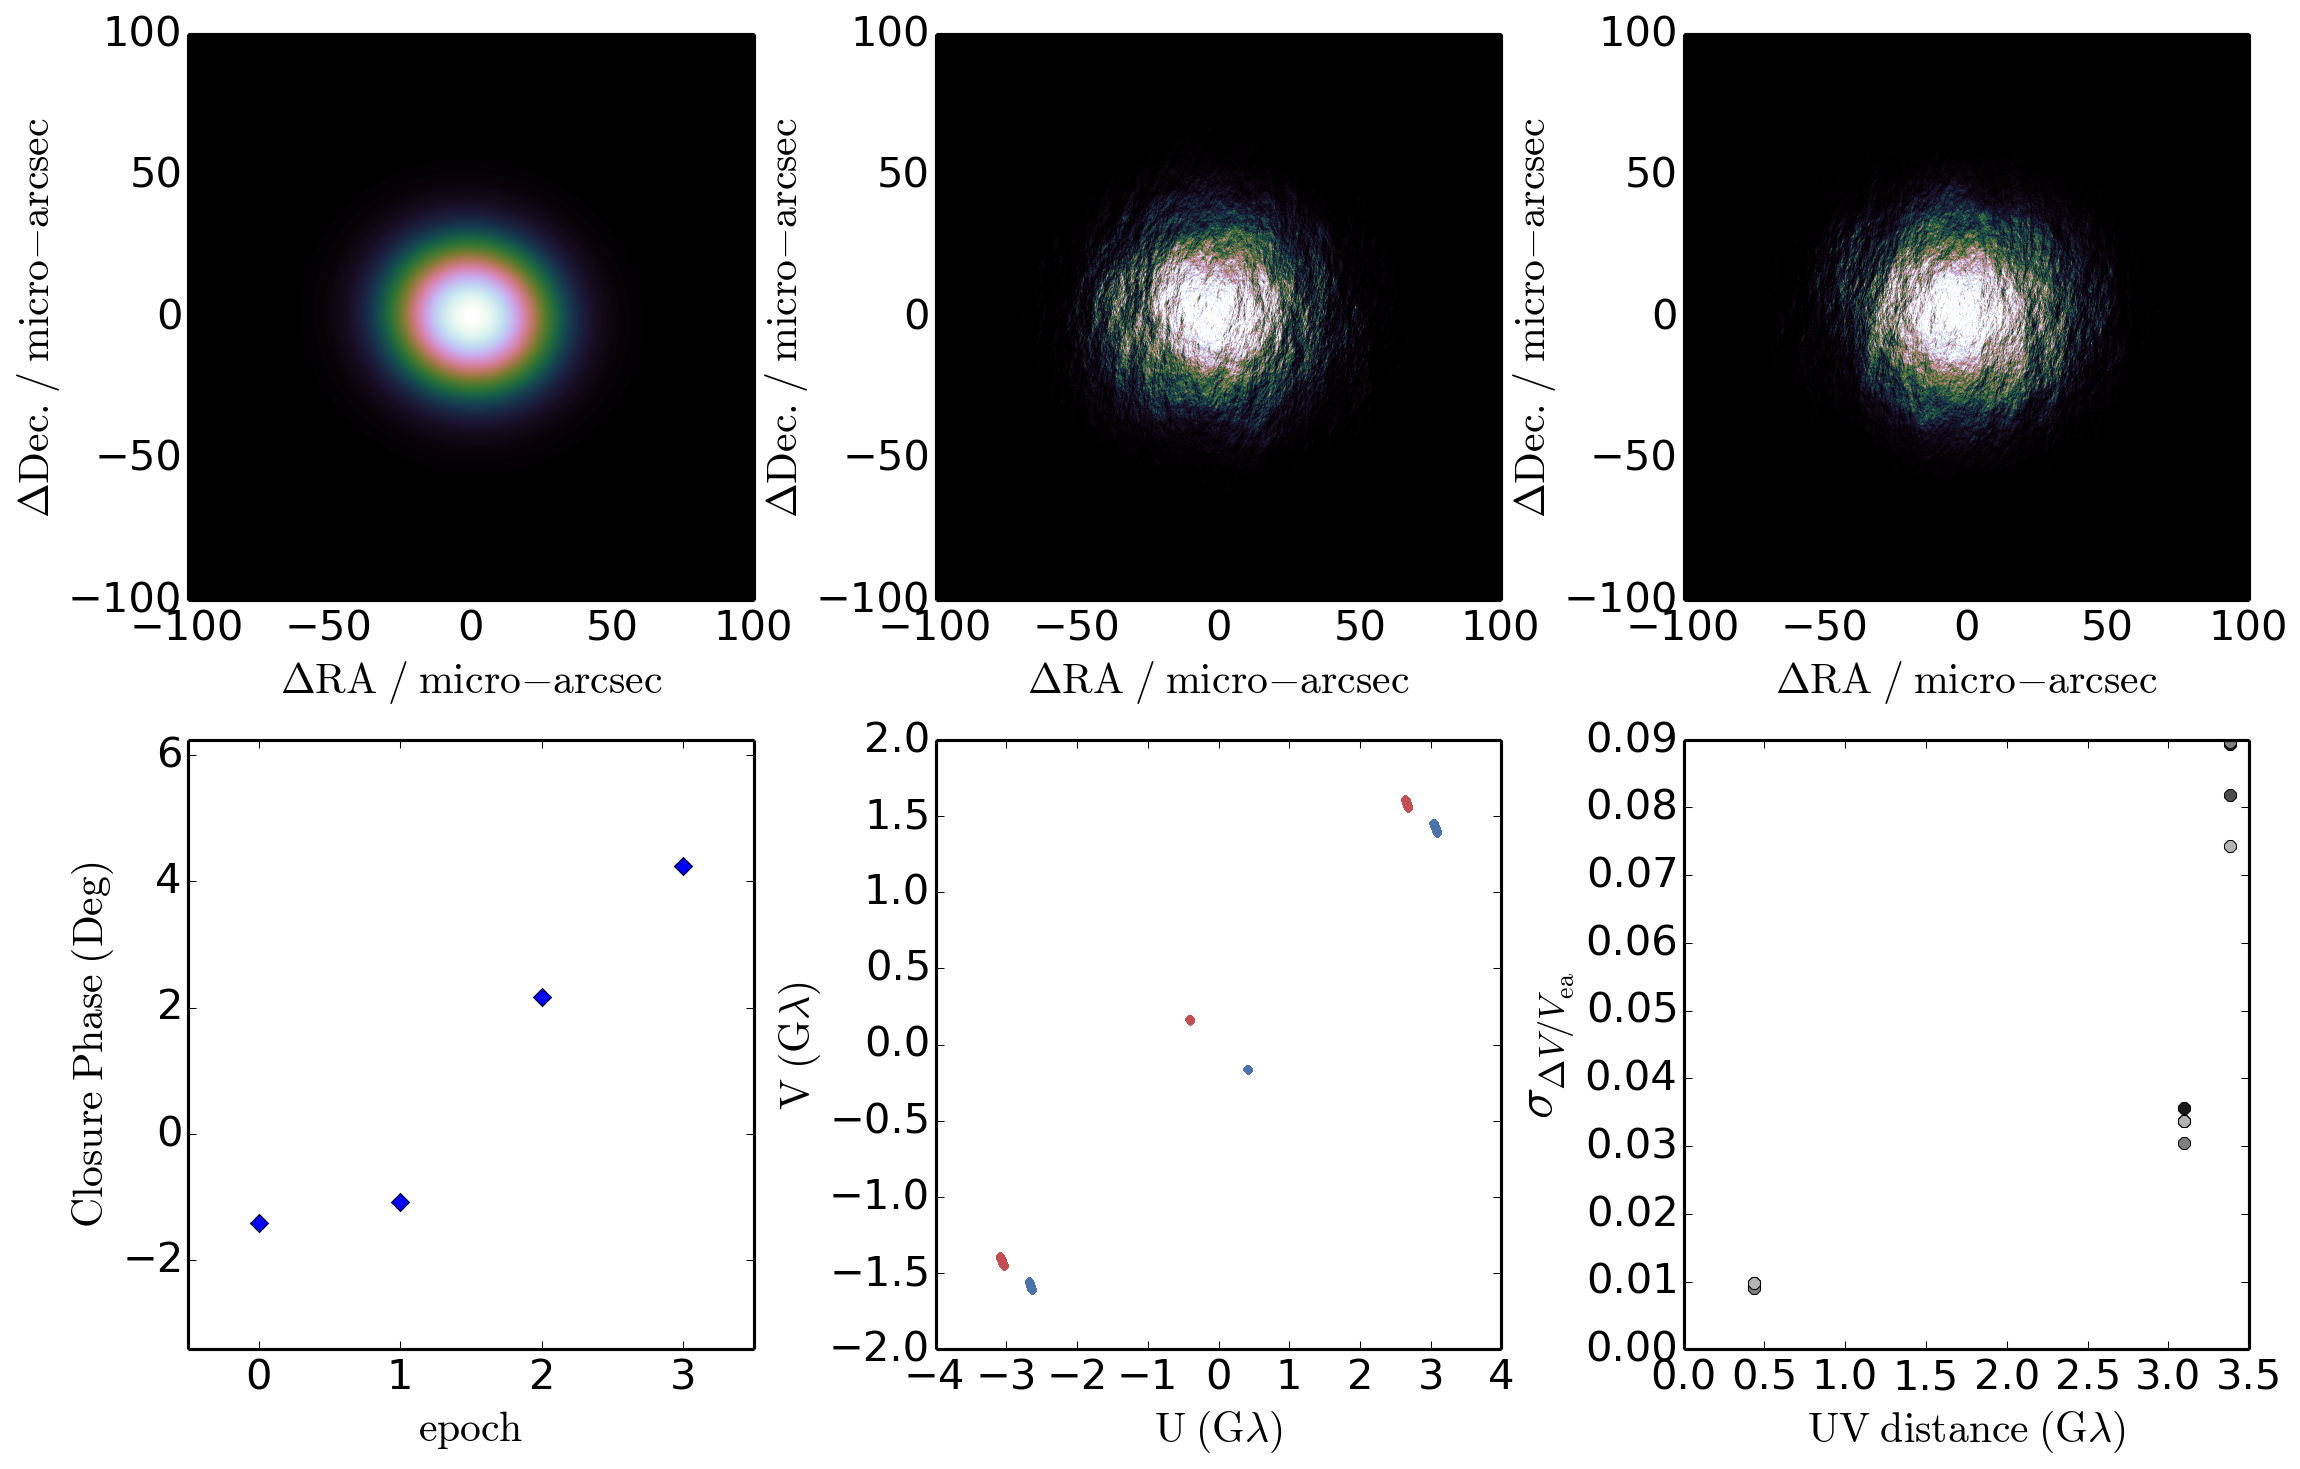
\includegraphics[width=\columnwidth]{Images/ism}
\caption{``An example simulation of ISM scattering towards Sgr~A$^{\star}$, observed with SMT-JCMT-CARMA.  The top panel, left to right, shows the original $\rm FWHM = 40$~$\mu$-arcsec Gaussian {\bf (top left)}, the simulated ISM scattered image on the first night {\bf (top middle)} and last night {\bf (top right)} of the observation, respectively.  The bottom panel, left to right,  shows the evolution of the 10 minute-averaged closure phase with epoch {\bf (bottom left)}, {\sl uv}-tracks for each night {\bf (bottom middle)} and the RMS fractional visibility amplitude differences $\sigma_{\Delta V /V_{\rm ea}}$ as a function of {\sl uv-}distance {\bf (bottom right)}. $ \Delta V= (|V_{\rm a}|-|V_{\rm ea}|)$, where $|V_{\rm a}|$ and $|V_{\rm ea}|$ are the simulated average and ensemble average visibility amplitudes respectively. Variations from the ensemble-average flux on the shortest baselines reveal total flux modulation while flux variations on longer baselines and non-zero closure phases track the fluctuations in substructure.''(Image and caption reproduced from \citet{Blecher_2016}) \label{ISM_sequence}%
}
\end{figure}

\subsubsection{Atmospheric transmission and scattering}

%st1
As described in section~\ref{sec:trop_imp}, the implementation of the tropospheric module is separated into mean and turbulent components. For the mean atmosphere, we simulate opacity, sky brightness temperature and time delay as a function of site weather, elevation angle and frequency. The most important climate parameters are precipitable water vapour column depth (PWV), ground temperature and ground pressure. The turbulent module simulates Guassian fluctuations in the time delay $\tilde{t}$ arriving at each station, where $\sigma(\tilde{t})$ is based on Kolmogorov turbulence on a two-dimensional scattering screen.


%Opacity + Brightness temperature st 1 - leave for now
The first atmospheric result we present are mean opacities and sky brightness temperatures for ALMA, the Submillimeter Array (SMA) and the South Pole Telescope (SPT) at 230~GHz, shown in Fig.~\ref{fig:mean_atm}. These sites were chosen as they are all considered excellent sites for sub-mm astronomy and form an essential part of the EHT. The PWV ranges used were taken from the 25th and 75th percentile data shown in \citet{Lane_1998} and is in good agreement with the measured opacities therein. %The ground% where I got the pressure/temp data from? I think it was SPT -lane 1998, ALMA - website/aatm defaults, SMA - site memo

%st 1
\begin{figure}[h!]
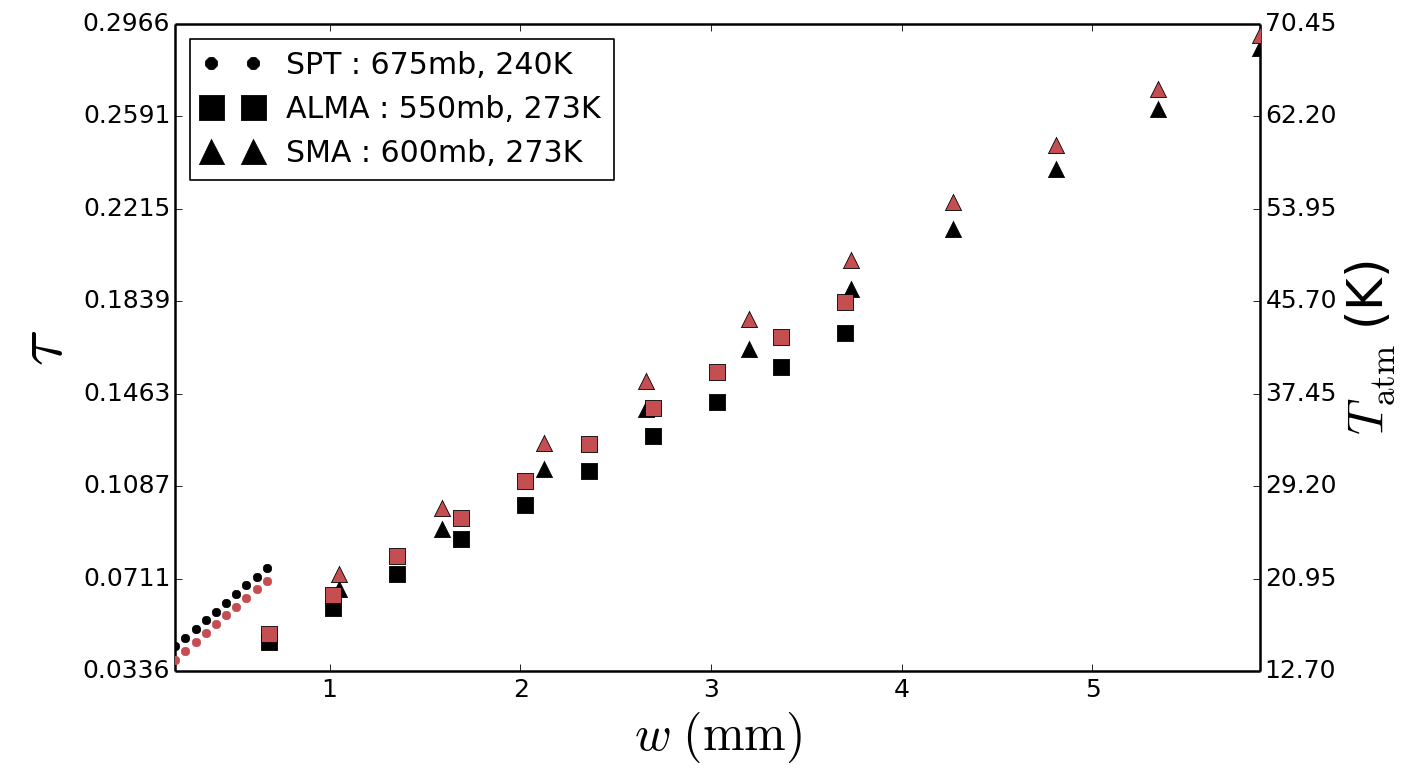
\includegraphics[width=1.\columnwidth]{Images/opacity}
\caption{``Simulated mean opacity (black) and sky brightness temperature (red) at $\nu =230$~GHz  for three typical ground pressures and temperatures over a typical PWV range \citep{Lane_1998} which approximately represent the sites of SPT (dots), ALMA (squares) and SMA (triangles). The legend shows the estimated input ground (pressure, temperature) parameters for each site.''(Image and caption reproduced from \citet{Blecher_2016})\label{fig:mean_atm}%
}
\end{figure}

%st 1 -a bit silly that I didnt do any 'bad' sites like PDBI or something like that
Immediately apparent is that the opacity and sky brightness temperature both exhibit linear relationships with respect to PWV content. Furthermore, opacity and sky brightness temperature are proportional to ground pressure and inversely proportional to the ground temperature \citep{Pardo_2001}. It is also clear that SPT has far less opacity, and a lower sky brightness temperature than ALMA and the SMA which are fairly similar. A comparison of the thermal receiver temperatures for the three sites  (ALMA$\sim262$~K,  SMA$\sim327$~K, SPT$\sim 255$~K) reveals that for the thermal noise contribution from the receiver is approximately an order of magnitude higher than sky brightness temperature. 



%Turbulent and mean delay st 1
Of vital importance to an interferometric site is atmospheric stability. An example of the effects of atmospheric transmission and scattering on the time delay $\tilde{t}$ at 230~GHz is shown as a function of observation time in Fig.~\ref{delay_plots}. Canonical values (see caption) were used for the weather parameters. It is apparent that the turbulent component is typically 3-4 orders of magnitude lower than the mean delay, even though the coherence time is on the order of seconds.


%st1
\begin{figure}[h!]
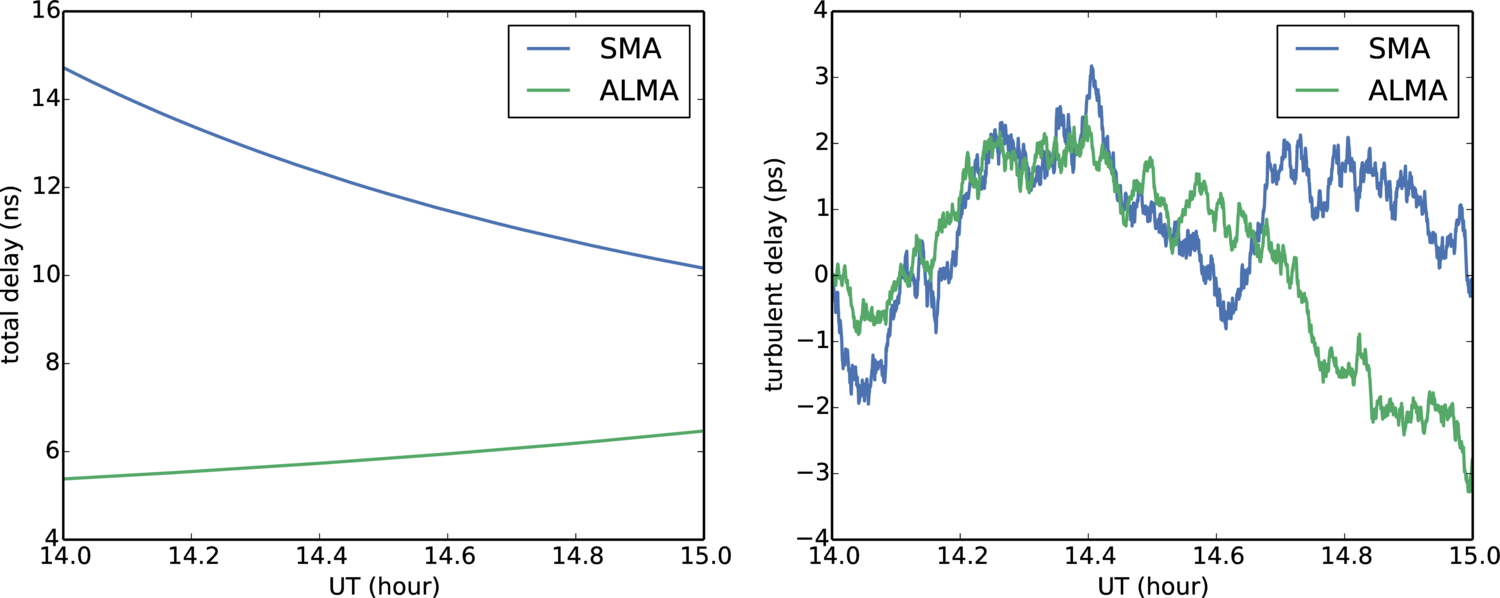
\includegraphics[width=\columnwidth]{Images/delays}
\caption{``Simulation of the total delay (left) and the turbulent atmospheric delay (right) for SMA (blue) and ALMA (green) sites towards Sgr~A$^\star$. Ground pressures and temperatures are the same as Fig.~\ref{fig:mean_atm}, precipitable water vapour above each station is set to $w=2$~mm, and the instantaneous zenith coherence time is set $T_0=10$~s for both stations. Note that all tropospheric parameters are, however, independently set. The conversion from time delay to phase at 230~GHz is $1$~rad~$=0.7$~ps.''(Image and caption reproduced from \citet{Blecher_2016})\label{delay_plots}%
}
\end{figure}



%Trop images
\begin{quotation}
``We now investigate the effect of the tropospheric module on image quality for various levels of calibration accuracy. We simulate the simple scenario of a sky model that consists of a 2.4~Jy point source at the phase centre, which is an approximate EHT-measured flux density of Sgr~A$^\star$ at 230~GHz. We assume a zenith phase coherence time of $t_0=10$~s above each station (however, each stations PWV can be independently simulated). We approximate the effect of imperfect calibration by adding a small fraction of the turbulent phase noise. For this example, we do not include the mean delay component, assuming it to be perfectly corrected for during the calibration. Imaging [is performed] using the two dimensional inverse fast Fourier transform''\\
\citep{Blecher_2016}
\end{quotation}

%Trop images
\begin{figure}[h!]
\includegraphics[width=\columnwidth]{Images/trop_images}
\caption{``The effect of residual troposphere phase noise on interferometric images of a point source observed for 12 hours at 230~GHz with 4~GHz bandwidth with the following array : SPT, ALMA, SMA, SMT, LMT and JCMT, assuming the same SEFDs as \protect\citet{Lu_2014} and an elevation limit of 15$^\circ$. For simplicity the weather parameters at each station were set to: coherence time $t_{\rm 0}=10$~sec; PWV depth $w=1$~mm; ground pressure $P=600$~mb; ground temperature $T =273$~K. {\bf Top left:} interferometric map with thermal noise only. {\bf Top right:} atmospheric attenuation and sky noise (due to non-zero opacity) with 1\% of the turbulent phase noise added. {\bf Bottom left:} as previous but with 3\% of turbulent phase contribution. {\bf Bottom right:} as previous but with 6\% turbulent phase contribution. The fractional turbulent phase contributions are illustrative of the effect of fringe-fitting errors. The black crosshairs indicate the original source position. ''(Image and caption reproduced from \citet{Blecher_2016}) \label{fig:trop_images}%
}
\end{figure}


%st 1 - attenuation of flux
Analysis of the images reveal increasing attenuation in the original peak, central flux due to the simulated residual calibration errors. In the calibration procedure, station gains cannot be solved for on arbitrarily short intervals as adequate SNR is needed to fringe-fit/self-calibrated. Aside from the fact that solutions are imperfect, within a given solution interval, there will also be a degree of uncalibrated turbulence-induced phase fluctuations.

Specifically, the flux of original central peak component is reduced to $76.5\%$ (attenuation only - not shown in plot), $75.1\%$ (1\% turbulence), 65.5\% (2\% turbulence) and  40.5\% (3\% turbulence). In the case of 3\% turbulence, the imaging artifact vertically below the source at 44.5\% of the original source flux becomes brighter than the corrupted source. 


%offset in original source st 1
Furthermore, there are slight offsets in the central peak flux from the original source position as shown by progressive movement away from the black crosshairs. This shift $\approx 5.6\ \mu$-arcsec at 3\% turbulence. 


%st 1
The residual calibration errors also distort the interferometric artifacts (as seen in the uncorrupted image), which result from inadequate sampling of the Fourier domain before imaging. This distortion causes a breakdown in image-plane deconvolution and source finding algorithms as the Point Spread Function (PSF) is difficult to subtract and the interferometric artefacts are difficult to distinguish from source structure. This further weakens the ability of such source finding algorithms to extract, with high fidelity, the BH shadow feature.


%Absence of blurring st 1
There was no evidence of blurring or a loss of resolution in the simulated images of Fig.~\ref{fig:trop_images}. Blurring can result if the decoherence is considered proportional to baseline length, as longer baselines would be less coherent and so their visibility amplitudes are effectively downweighted. For the EHT, as different stations experience completely independent phase fluctuations, the baseline length of the VLBI baselines will not be correlated with the magnitude of the decoherence. Alternatively, the blurring consequence, characteristic in optical single dish telescopes as 'seeing', is induced by the overlaying of many speckled images of the source \citep{Narayan_1992} across the scattering disc. This does not seem to occur in the interferometric image reconstruction with the inverse fourier transform. The reason being that the phase noise of each fourier mode is Gaussian, and so positional deviations of each Fourier mode from zero phase noise effectively cancel in the image domain. Hence attentuation but no blurring.


%Incoherent closure phases.. This section is needed to link up to the discussion on closure phase uncertainty in the mm-VLBI section. Yep worth mentioning. but leave this 

%NON-CLOSING ERRORS
%Non-closing errors due to incoherent averaging - "no conjugates for triples" - possibly comes down to how one defines SNR. In the definition used in the literature we followed, they assumed only gaussian noise, which was not the case..A better definition would be to look at the distribution of a number of samples 
%maybe just a mention of how the closure phase uncertainty could change.

\subsubsection{Antenna pointing offset}

%mild intro


\begin{quotation}
``We investigate the effect of pointing errors on the 50~m (i.e. fully illuminated) Large Millimeter Array (LMT) dish configured in an eight station VLBI array. The LMT has been measured to have an absolute pointing accuracy of $\sigma_{\rm abs} = 1-3$~arcsec, where smaller offsets occur when observing sources closer to zenith, and a tracking pointing accuracy $\sigma_{\rm track} < 1$~arcsec\footnote{http://www.lmtgtm.org/telescope/telescope-description/}. We investigate the observational effect of these errors through three different pointing error models which explore different instructive and plausible scenarios. The LMT has been singled out due to its narrow primary beam and that it may serve as a reference station for the EHT array given its sensitivity and central geographic location. 

The source used is a circular Gaussian of characteristic size $\Theta_{\rm src}=50$ $\mu$-arcsec, located at the phase centre. For this investigation, as long as $\Theta_{\rm src} \ll \theta_{\rm PB}$, the exact structure of the source is unimportant. We approximate the LMT beam profile using an analytic WSRT beam model (equation~\ref{eq:wsrt_beam}) with a factor of two increase in the beam factor $C$ to take into account the increased dish size of the LMT. [Hence] $C_{\rm LMT} \approx 130$~GHz$^{-1}$. Note that the power beam $EE^H$ becomes $\cos^6$, resulting in a $\rm{FWHM} = 6.5 $~arcsec at 230 GHz.


We make use of the RMS fractional visibility amplitude error $\sigma_{\Delta V/V_0}$, where $V_{\rm PE}$ and $V_{0}$ are the visibility amplitudes with and without pointing errors respectively, and  $\Delta V = V_{\rm PE} - V_{0}$.
\\
\citep{Blecher_2016}
\end{quotation}

%the different pointing models
For this simulation we use three different pointing error models, as introduced in section~\ref{sec:instrument}. Firstly, we simulate a simple \emph{constant} pointing offset. For the second case, we simulate a smooth, \emph{sinusoidal} pointing error to replicate a tracking error. The period of the sinusoid is sampled from a uniform distribution between 0.5 and 6 hours, and a peak amplitude $A_{\rho} = \sqrt{2} \sigma_{\rho}$ , where the factor $\sqrt{2}$ relates the peak amplitude to the RMS of a sinusoidal, zero-mean waveform.  In the third case, we simulate \emph{stochastic} variability which replicates slewing from source/calibrator to source/calibrator, where the pointing error is re-sampled every 10 minutes from a Gaussian of characteristic width equal to the quoted pointing error. This simulation is repeated for 50 realisations for each pointing offset to generate reasonable uncertainties \citep{Blecher_2016}. In Fig.~\ref{fig:pointing}, $\sigma_{\Delta V/V_0}$ is plotted against pointing error $\rho$ over the range $0 \le \rho \le 4.5$~arcsec for the three classes of error. Note that although plotted on the same set of axes, $\rho$ represents slightly different quantities for each of the three simulations.

%analysis : why LMT, and phased array
\begin{quotation}
``We only consider LMT pointing errors due to its narrow primary beam and potential to be used as a reference station. However, the capability to simulate independent pointing errors for each station is available. In the case of a phased array, a pointing error simulation could be used to investigate the contribution of the pointing error to a variable phasing efficiency, which can be reasonably approximated by a scalar Jones matrix.''\\
\citep{Blecher_2016}
\end{quotation}


\begin{figure}[h!]
\includegraphics[width=\columnwidth]{Images/point_Crop}
\caption{``RMS relative amplitude error induced by pointing error with the 50~m (i.e. fully illuminated) LMT antenna as a function of pointing error offset $\rho$ at 230~GHz. We assume that these errors are degenerate or non-separable from the self-calibration/fringe-fitting model used. See text for the description of the three models used. This simulation capability enables constraints on the magnitude of pointing-induced errors given a particular pointing calibration strategy.''(Image and caption reproduced from \citet{Blecher_2016})\label{fig:pointing}%
}
\end{figure}
\

\begin{quotation}
``Visibility amplitude errors due to antenna pointing error has been investigated for the $50$~m  LMT dish operating at $230$~GHz. In Fig.~\ref{fig:pointing}, we show that pointing errors associated with frequent phase centre switching (stochastic variability) could introduce a RMS fractional amplitude error $\sigma_{\Delta V/V_0} \sim 0.1 - 0.4$ for an absolute pointing accuracy  $\sigma_{\rm abs} \sim 1-3$~arcsec. In contrast, tracking errors are less problematic with $\sigma_{\Delta V/V_0} \le 0.05$ for a tracking accuracy  $\sigma_{\rm track}<1$~arcsec. The case of a constant error pointing model is comparable to that of the `slow variability' case. If the gain error is non-separable from the calibration model used, it could be interpreted as intrinsic variability, substructure and/or increased noise. If unaccounted for, this effect has the potential to limit the dynamic range of mm-VLBI images. Further tests to constrain the pointing uncertainties of EHT stations will lead to more accurate interferometric simulations and hence the overall impact on black hole shadow parameter estimation. Here we demonstrate the capability to incorporate a range of plausible pointing error effects into a full simulation pipeline. For future observations at 345~GHz, these effects will be even more pronounced, given the narrower primary beam.\\
\citep{Blecher_2016}
\end{quotation}





%\subsubsection{Performance?}
%Performance/speed



%\section{Fringe-fitting test}
%leave until done
%First we fringe fit and image a stationary point source and compare to the result in Fig.~\ref{fig:trop_images}. 
% In an upcoming paper, we perform a systematic exploration of the turbulent tropospheric effects on the accuracy of fringe-fitting algorithms/strategies, through use of an automated calibration procedure and including the added complexity of a time-variable source.


\section{Suggested applications and improvements}\label{sec:improv}

\subsubsection{Anomalous pointing error}
There is another class of pointing error which we did not include in our simulation, but which could be folded in through a combination of the tropospheric and antenna pointing modules. This is the so-called `anomalous pointing error' and is due to the time-variable phase-gradient across the aperture \citep[e.g.][]{Holdaway_1997,Butler_1997,Holdaway_1998}. This is essentially the first order fluctuation in water vapour across the antenna and hence will be proportional to the structure function evaluated at the dish diameters. These are pointing errors which will change on the timescale $d_{\rm dish}/v \sim 1-50$~s for $10<d_{\rm dish}<50$~m and $1<v<10$~m/s, where $d_{\rm dish}$ is the diameter of the aperture.  

\citet{Holdaway_1998} derives the standard deviation of the pointing error as a fraction of beam width,
\begin{equation}
 \sigma_{\rm pe}(d_{\rm dish}),\theta) = \frac{\sqrt{2} \sigma_l(d_{\rm dish)}}{\sqrt{\sin\theta}\lambda},
\end{equation}
where $\sigma_l(d_{\rm dish)} = \sqrt{D_l(d_{\rm dish}}$ is the standard deviation of path length fluctuations over the antenna diameter and $\theta$ is the elevation angle. Hence in terms of fractional beam size, the effect goes as $D^{\beta/2}$ and hence the effect for large dishes will be larger amplitude variations (as shown by Fig.~\ref{fig:pointing}) over longer time periods. 


Estimates of $\sigma_{\rm pe}$ shown in \citet{Holdaway_1998} range between $0.48-3.68$-arcsec, where the lower bound was calculated for an 8m dish, observing at zenith with relatively stable atmosphere and the upper bound was calculated for a 15m dish observing at $10^\circ$ with a relatively unstable atmosphere.  

Apertures which are fitted with radiometers are able to track the PWV distribution across the primary beam \citep{Lamb_1998}. However, most of the EHT station are currently not fitted with radiometers and hence this effect could be tricky to calibrate.

\subsubsection{Testing calibration, imaging and parameter estimation}

%Testing and development of calibration, imaging and parameter estimation pipelines st 1
The primary use of synthetic data is to provide 'known' datasets on which to run calibration, imaging and parameter estimation pipelines. This can take the form of beauty contests, where various algorithms are utilised without knowledge of the true source and the results are compared post-facto. This is especially useful with imaging algorithms which have many `hand-tuned' parameters and difficulty with repeatability, uniqueness and fidelity of their solutions. Alternatively, one could perform a more systematic investigation of how an algorithm performs under a range different conditions. A key test which we have alluded to throughout this thesis is a systematic exploration of the turbulent tropospheric effects on the accuracy of fringe-fitting algorithms/strategies, including the added complexity of a time-variable source. A key point of such an investigation being the capability of assigning quantitative values to systematic and stochastic uncertainties across a wide range of physically relevant conditions.


%bayesian calibration
%An original motivation for the {\sc meqsilhouette} simulator was that it could eventually be implemented as a bayesian calibration routine where the signal corruptions were solved for. However, as many of the dominant signal corruptions have turned out to be stochastic and hence indeterminant, it no longer makes sense to go down this route. Indeed one would need a GPU-accelerated simulator to be able to sample the parameter space. Fortunately then, a collegue is planning a GPU bayesian calibration routine.  

%end-to-end st 2 - but you dont need an end- to end for some of this - but good enough 
With the current work developing automated fringe-fitters at JIVE (casa-based) and UCT/SKA-SA (bayesian) by Des Small and Iniyan Natarajan respectively, there arises the possibility of an end-to-end simulation pipeline, i.e. from theory to calibrated data product, within the next year. In this scenario, one could estimate the precision and accuracy with which the EHT could extract parameters (e.g. shadow size and asymmetry) in a range of canonical scenarios. This will also allow weak points in the calibration/analysis to be identified and subsequently improved as well as to determine which approaches to extracting science are more viable (e.g. analysis in the visibility domain vs image domain).
This argument can be extended to the realm of station upgrades (e.g. enhanced bandwidth) and the investigation into novel (sub)millimetre sites. 


%Data interpretation st1
As the EHT will be observing in a unique regime, there will always be doubt, double-checking and questioning of the interpretation of the data. This is especially the case with the use of closure quantities, where the recent result of an increase in closure phase with UT hour, measured on the Hawaii-Arizona-California triangle \citep{Fish_2016}, provides a good example. Simulations help formulate and test quatitatively plausible scenarios. For example the contribution of different components (e.g. ISM substructure, SNR) to the scatter in this result could be investigated for different source models. 

\begin{quotation}
``Significant progress has been made in the theoretical and numerical modeling of the inner accretion flow and jet launch regions near a supermassive black hole event horizon
\citep[e.g.][]{Zanna_2007,Etienne_2010,Dexter_2013,Moscibrodzka_2014, McKinney_2014}. As the sensitivity of the EHT stands to dramatically increase, these theoretical efforts must be complemented by advances in interferometric simulations. With \textsc{MeqSilhouette}, we now have the ability to couple these with sophisticated interferometric and signal propagation simulations.  Moreover, detailed interferometric simulations will enable us to quantify systematic effects on the black hole and/or accretion flow parameter estimation.''\\
\citep{Blecher_2016}
\end{quotation}



\subsubsection{A public online interface}
%st 1
Table~\ref{tab:parameters} shows the set of parameters needed to run a standard {\sc meqsilhouette} simulation. This moderate number of parameters ($24+6N_{\rm stations}$) can be quickly chosen or selected from a list, especially if most of the defaults are preset and unlikely to change. This speaks to the possibility of an online GUI interface which would provide the user with the capability to run standard simulations without having to delve into code. The capability to run such simulations would be useful to both theorists and observers in the broader AGN/SMBH/mm-VLBI community. For this reason, we trialed an online interface at the Leiden 2015 mm-VLBI workshop\footnote{http://www.astron.nl/other/workshop/mm-VLBI2015} with an early version of the {\sc meqsilhouette} simulator, which was well received by the researchers present. We are, however, yet to convert the latest version of the pipeline \citep{Blecher_2016} into such an interface, but hopefully this implementation will be made available in the future when matters relating to public/propriety status of the codebase are cleared up.


\subsubsection{Full Stokes}
%st 1
One of the key observables for the EHT is polarisation dependent quantities \citep{Johnson_2015b}. Although this version focused only on total intensity, if {\sc meqsilhouette} is taken up by members of the community, subsequent versions will enable the full Stokes cube as input. This should not entail much work as our chosen data formats (MS, {\sc fits}) as well as the FFT and UV sampling routine in {\sc MeqTrees} already support full Stokes logic including parallactic angle rotation. Signal propagation through the ISM and troposphere as well as antenna based complex gains errors are polarisation independent. The work would be primarly involve altering the existing scripts to deal with the book-keeping of the extra dimension. In addition the implementation of the associated signal corruption, polarisation leakage, is straightforward in the RIME formalism as it is simply an off-diagonal Jones matrix which is approximately constant over the course of an observation.

%\subsubsection{Opacity and atmospheric brightness temperature fluctuations}
% basically 
%In addition to tropospheric turbulence-induced phase errors, the turbulent contribution to variations in opacity is also important.
%Run multiple realisations of atm to link the phase fluctuations to opacity and brightness temperature fluctuations %possibly by fluctuating the input climate parameters., but this might be unfeasible.


























%\chapter{Conclusion} %synthesis not summary..distill key and best ideas: 

%intro
In light of upcoming EHT observations and science goals as well as software advances in the broader radio interferometry community, a mm-VLBI data simulator has been developed as described first in \citet{Blecher_2016} and expanded upon in this thesis.

%link to design objectives
We believe that our design objectives, laid out in section~\ref{sec:des_obj}, are met from the diversity of simulations shown by our results. This work provides the most sophisticated data simulator for the EHT to date due to the implementation of several dominant physically-based signal corruptions and the generality of framework used. Even though the foundation of the simulator has been built, it is only through collaboration with the various EHT working groups that its potential will truly be achieved.


%data formats
The focus has been placed on simulating realistic data given an arbitrary theoretical sky model. The pipeline uses the {\sc Measurement Set} format, in line with ALMA and future VLBI data formats. However, there are various other data formats currently in use, due to shortcomings of the {\sc ms} with respect to mm-VLBI which still need attention. 


%experimental setup
We have focused on EHT observations, however, the pipeline is completely general with respect to observation configuration and allow any source structure in the form of {\sc fits} format e.g. through inclusion of an ionospheric module, simulations of low-frequency observations (e.g. with LOFAR) can be performed. 
%time variability
Time variability in all domains (source, array, ISM, troposphere) is implemented. We highlight this point as we view the development of calibration and imaging routines which deal appropriately with source variability an essential challenge for observations of Sgr~A* and M87. Distinguising complex gain variations, i.e. $\bm G$-Jones terms from short intrinsic variability will depend on the SNR obtained, where the inclusion of ALMA in the array will be pivotal in this regard. Software advances can also add further utility and aid in the construction of a high precision instrument. A synthetic data simulator could prove essential to research and test calibration, imaging and parameter estimation strategies.
%corruptions & formalism
To this end, the simulator includes signal corruptions in the interstellar medium (ISM), troposphere and instrumentation. Examples of typical corruptions have been demonstrated, which show that each corruption can significantly affect the inferred scientific parameters. A wide range of signal propagation effects can be implemented using the Measurement Equation formalism, and the simulator can be easily extended to include bandpass imperfections and polarisation leakage.
%SPECIFIES, VALUES etc


%ISM
The ISM scattering implementation \textsc{ScatterBrane}, based on \citet*{Johnson_2015a}, has been incorporated into the pipeline.
%ISM - 4 day
We have shown an intuitive example of how ISM substructure and variability in the average regime is different to the purely deterministic Gaussian-blurring effect of the ensemble-average regime (Fig.~\ref{ISM_sequence}). This was explored through multiple observables, including the appearance of the scattered image, the closure phase and visibility amplitude.
%ISM cp envelope
In addition to this, we have also shown that the ISM module has statisical power by reproducing the ISM-induced closure phase uncertainty envelope calculated in \citet{Ortiz_2016}, shown in Fig.~\ref{fig:substructure2}.
%ISM general
We have discussed how ISM substructure and variability can be difficult to disentangle from the instrinsic source structure, especially if the source is also variable. The magnitude of the refractive substructure will depend on the size of the emission region which at 1.3~mm is sensitive to optical depth effects due to synchrotron self-absorption and accretion history. If possible, observations of Sgr~A* should ideally be spaced apart by $r_{\rm ref}/v \sim$ a week in order to sample independent realisations of the scattering screen. 

%mean trop
We have taken a unique approach to separate the atmosphere in mean and turbulent components. In the mean component, we perform a sophisticated radiative transfer calculation using the {\sc atm} software, with an example calculation for three millimetre sites over a range of weather conditions shown in Fig.~\ref{fig:mean_atm}.
%trop im
For the turblent model, we employ Kolmogorov, thin-screen statisics to simulate independent phase corruptions for each station. Where we simulated images of a point sources with residual calibration errors, we find rapidly increasing flux attenuation from 1\% at 1\% turbulence to 36\% at 6\% turbulence. Tropospheric phase noise also distorts the typical interferometric response or PSF in the image which could cause difficulties in source extraction. We also find a centroid offset of $\approx 5.6\ \mu$-arcsec at 6\% turbulence, which could be difficult to separate from source variability.


%antenna pointing
We have simulated the effects of antenna pointing error models corresponding to tracking and slew errors on the LMT. We find that slewing introduces large fraction visibility amplitude errors $\sigma_{\Delta V/V_0} \sim 0.1 - 0.4$ while tracking introduces smaller errors $\sigma_{\Delta V/V_0} \le 0.05$ but still large enough to significant in the larger uncertainty budget. Furthermore, we have briefly discussed the effects of the turbulent atmosphere on antenna pointing. This `anomalous' pointing error is potentially a serious calibration difficulty for sites without radiometers, and systematic simulations are recommended to quantify this further. 

%
Applications for which the current version of the pipeline is well suited for include testing calibration and imaging routines in total intensity. One example which we have discussed is fringe-fitting in the presence of a variable troposphere with time-variable source.  
The creation of a close interface between sophisticated theoretical and interferometric mm-VLBI simulations will enhance the scientific opportunities possible with the EHT. 

%future
As the development of {\sc meqsilhouette} continues, future capabilities will include full Stokes capability including polarised sky models and polarisation leakage as well as the simulation of pointing errors due to `anomalous refraction'.  To promote connection between theory and data, a standard version of {\sc meqsilhouette} could be run through an online interface. This would make interferometric simulations public or available to the mm-VLBI community.  















\bibliography{thesis}
\bibliographystyle{plainnat}
\addcontentsline{toc}{chapter}{Bibliography}

\end{document}
